%\documentclass[a4paper,11pt]{book}
\documentclass[a4paper,twoside,11pt,titlepage]{book}
\usepackage{listings}
\usepackage[utf8]{inputenc}
\usepackage[spanish]{babel}
\usepackage{fullpage, mathpazo, amsmath, amsthm, amssymb, amsfonts, nicefrac}
\usepackage{vmargin}

\usepackage{cite}

% \usepackage[style=list, number=none]{glossary} %
%\usepackage{titlesec}
%\usepackage{pailatino}

\decimalpoint
\usepackage{dcolumn}
\newcolumntype{.}{D{.}{\esperiod}{-1}}
\makeatletter
\addto\shorthandsspanish{\let\esperiod\es@period@code}
\makeatother


%\usepackage[chapter]{algorithm}
\RequirePackage{verbatim}
%\RequirePackage[Glenn]{fncychap}
\usepackage{fancyhdr}
\usepackage{graphicx}
\usepackage{afterpage}

\usepackage{longtable}

\usepackage[pdfborder={000}]{hyperref} %referencia

% ********************************************************************
% Re-usable information
% ********************************************************************
\newcommand{\myTitle}{Geometría y Visualización\xspace}
\newcommand{\myDegree}{Máster en Matemáticas\xspace}
\newcommand{\myName}{Jesús Bueno Urbano\xspace}
\newcommand{\myProf}{Carlos Ureña Almagro\xspace}
\newcommand{\myOtherProf}{Pedro A. García Sánchez\xspace}
%\newcommand{\mySupervisor}{Put name here\xspace}
%\newcommand{\myFaculty}{Your Faculty here\xspace}
%\newcommand{\myFacultyShort}{\xspace}
%\newcommand{\myDepartment}{Your department here\xspace}
\newcommand{\myUni}{\protect{Universidad de Granada}\xspace}
%\newcommand{\myLocation}{Granada\xspace}
%\newcommand{\myTime}{\today\xspace}
%\newcommand{\myVersion}{Version 0.1\xspace}


\hypersetup{
pdfauthor = {\myName},
pdftitle = {\myTitle},
pdfsubject = {},
pdfkeywords = {}
pdfcreator = {TeX Live},
pdfproducer = {pdflatex}
}

%\hyphenation{}


%\usepackage{doxygen/doxygen}
%\usepackage{pdfpages}
\usepackage{url}
\usepackage{colortbl,longtable}
\usepackage[stable]{footmisc}
%\usepackage{index}

%\makeindex
%\usepackage[style=long, cols=2,border=plain,toc=true,number=none]{glossary}
% \makeglossary

% Definición de comandos que me son útiles:
%\renewcommand{\indexname}{Índice alfabético}
%\renewcommand{\glossaryname}{Glosario}

\pagestyle{fancy}
\fancyhf{}
\fancyhead[LO]{\leftmark}
\fancyhead[RE]{\rightmark}
\fancyhead[RO,LE]{\textbf{\thepage}}
\renewcommand{\chaptermark}[1]{\markboth{\textbf{#1}}{}}
\renewcommand{\sectionmark}[1]{\markright{\textbf{\thesection. #1}}}

\setlength{\headheight}{1.5\headheight}

\newcommand{\HRule}{\rule{\linewidth}{0.5mm}}
%Definimos los tipos teorema, ejemplo y definición podremos usar estos tipos
%simplemente poniendo \begin{teorema} \end{teorema} ...
\theoremstyle{definition}
\newtheorem{definition}{Definición}[section]
\newtheorem{lemma}{Lema}[section]
 
\theoremstyle{remark}
\newtheorem*{remark}{Nota}

\definecolor{gray97}{gray}{.97}
\definecolor{gray75}{gray}{.75}
\definecolor{gray45}{gray}{.45}
\definecolor{gray30}{gray}{.94}

\lstset{ frame=Ltb,
     framerule=0.5pt,
     aboveskip=0.5cm,
     framextopmargin=3pt,
     framexbottommargin=3pt,
     framexleftmargin=0.1cm,
     framesep=0pt,
     rulesep=.4pt,
     backgroundcolor=\color{gray97},
     rulesepcolor=\color{black},
     %
     stringstyle=\ttfamily,
     showstringspaces = false,
     basicstyle=\scriptsize\ttfamily,
     commentstyle=\color{gray45},
     keywordstyle=\bfseries,
     %
     numbers=left,
     numbersep=6pt,
     numberstyle=\tiny,
     numberfirstline = false,
     breaklines=true,
   }
 
% minimizar fragmentado de listados
\lstnewenvironment{listing}[1][]
   {\lstset{#1}\pagebreak[0]}{\pagebreak[0]}

\lstdefinestyle{CodigoC}
   {
	basicstyle=\scriptsize,
	frame=single,
	language=C,
	numbers=left
   }
\lstdefinestyle{CodigoC++}
   {
	basicstyle=\small,
	frame=single,
	backgroundcolor=\color{gray30},
	language=C++,
	numbers=left
   }

 
\lstdefinestyle{Consola}
   {basicstyle=\scriptsize\bf\ttfamily,
    backgroundcolor=\color{gray30},
    frame=single,
    numbers=none
   }


\newcommand{\bigrule}{\titlerule[0.5mm]}


%Para conseguir que en las páginas en blanco no ponga cabeceras
\makeatletter
\def\clearpage{%
  \ifvmode
    \ifnum \@dbltopnum =\m@ne
      \ifdim \pagetotal <\topskip
        \hbox{}
      \fi
    \fi
  \fi
  \newpage
  \thispagestyle{empty}
  \write\m@ne{}
  \vbox{}
  \penalty -\@Mi
}
\makeatother

\usepackage{pdfpages}
\renewcommand{\baselinestretch}{1.25} %Interlineado
\begin{document}
\begin{titlepage}
 
 
\newlength{\centeroffset}
\setlength{\centeroffset}{-0.5\oddsidemargin}
\addtolength{\centeroffset}{0.5\evensidemargin}
\thispagestyle{empty}

\noindent\hspace*{\centeroffset}\begin{minipage}{\textwidth}

\centering

\includegraphics[width=0.9\textwidth]{images/logo_ugr.png}\\[1.4cm]

\textsc{ \Large TRABAJO FIN DE MÁSTER\\[0.2cm]}
\textsc{Escuela Internacional de Posgrado}\\[1cm]
% Upper part of the page
% 
% Title
{\Huge\bfseries Geometría y visualización\\
}
\noindent\rule[-1ex]{\textwidth}{3pt}\\[3.5ex]
%{\large\bfseries Subtitulo del Proyecto}
\end{minipage}

\vspace{2.5cm}
\noindent\hspace*{\centeroffset}\begin{minipage}{\textwidth}
\centering

\textbf{Autor}\\ {Jesús Bueno Urbano}\\[2.5ex]
\textbf{Directores}\\
{Carlos Ureña Almagro\\
Pedro A. García Sánchez}\\[2cm]

\includegraphics[width=0.3\textwidth]{images/mm.pdf}\\[0.1cm]
\textsc{Máster Universitario en Matemáticas}\\
\textsc{---}\\
Granada, 2018
\end{minipage}
%\addtolength{\textwidth}{\centeroffset}
%\vspace{\stretch{2}}
\end{titlepage}



%\chapter*{}
%\thispagestyle{empty}
%\cleardoublepage

%\thispagestyle{empty}

%\begin{titlepage}
 
\thispagestyle{empty}
\setlength{\centeroffset}{-0.5\oddsidemargin}
\addtolength{\centeroffset}{0.5\evensidemargin}
\thispagestyle{empty}

\noindent\hspace*{\centeroffset}\begin{minipage}{\textwidth}

\centering
%
\includegraphics[width=0.9\textwidth]{images/logo_ugr.png}\\[1.4cm]



 \vspace{3.3cm}

%si el proyecto tiene logo poner aquí

\includegraphics{images/mm.pdf} 
 \vspace{0.5cm}

% Title

{\Huge\bfseries Geometría y visualización\\
}
%\noindent\rule[-1ex]{\textwidth}{3pt}\\[3.5ex]
%{\large\bfseries Subtítulo del proyecto.\\[4cm]}
\end{minipage}

\vspace{2.5cm}
\noindent\hspace*{\centeroffset}\begin{minipage}{\textwidth}
\centering

\textbf{Autor}\\ {Jesús Bueno Urbano}\\[2.5ex]
\textbf{Directores}\\
{Carlos Ureña Almagro\\
Pedro A. García Sánchez}\\[2cm]
%\includegraphics[width=0.15\textwidth]{images/tstc.png}\\[0.1cm]
%\textsc{Departamento de Teoría de la Señal, Telemática y Comunicaciones}\\
%\textsc{---}\\
%Granada, mes de 201
\end{minipage}
%\addtolength{\textwidth}{\centeroffset}
\vspace{\stretch{2}}

 
\end{titlepage}






\cleardoublepage
\thispagestyle{empty}

\begin{center}
{\large\bfseries Geometría y visualización}\\
\end{center}
\begin{center}
Jesús Bueno Urbano\\
\end{center}

%\vspace{0.7cm}
%\noindent{\textbf{Palabras clave}: palabra\_clave1, palabra\_clave2, palabra\_clave3, ......}\\

\vspace{0.7cm}
\noindent{\textbf{Resumen}}

En este Trabajo Fin de Máster hemos querido hacer un recorrido por los conceptos básicos de del Ray Tracing para poder representar y visualizar superfícies implícitas. Para ello en el  primer capítulo haremos un repaso sobre métodos elementales para implicitar superficies, es decir, para poder transformar una expresión no implícita, paramétrica en nuestro caso, de una superficie en la expresión implícita de ésta. Sobre todo nos centraremos en el método de la base de Gröbner y presentaremos los métodos de la resultante y de Wu-Ritt.

Ya en el segundo capítulo el tema principal de éste será buscar métodos de visualización de superficies como la poligonalización de superficies, en particular, presentaremos un algoritmo de triangulación extraído de \cite{Hartmann03}. A continuación explicaremos el concepto de Ray Tracing.

A continuación haremos una introducción al Análisis de Intervalos y a sus propiedades, a los Intervalos Modales y a las llamadas extensiones semánticas. Todo esto nos servirá para, finalmente, aplicarlo al Ray Tracing y así presentar varios algoritmos mejorados cuya eficiencia compararemos.
\cleardoublepage


%\thispagestyle{empty}


%\begin{center}
%{\large\bfseries Project Title: Project Subtitle}\\
%\end{center}
%\begin{center}
%First name, Family name (student)\\
%\end{center}

%\vspace{0.7cm}
%\noindent{\textbf{Keywords}: Keyword1, Keyword2, Keyword3, ....}\\

%\vspace{0.7cm}
%\noindent{\textbf{Abstract}}\\

%Write here the abstract in English.

\chapter*{}
\thispagestyle{empty}

\noindent{\rule[-1ex]{\textwidth}{2pt}\\[4.5ex]}
Yo, \textbf{Jesús Bueno Urbano}, estudiante del Máster Universitario en Matemáticas de la \textbf{Escuela Internacional de Posgrado de la Universidad de Granada}, con DNI 20078941X, autorizo que la siguiente copia de mi Trabajo Fin de Máster pueda ser consultada por las personas que lo deseen.

\vspace{2cm}


\includegraphics[scale=0.3]{images/firma.png}

\vspace{1cm}

\noindent Fdo: Jesús Bueno Urbano

\vspace{2cm}

\begin{flushright}
En Granada, a \today.
\end{flushright}


\chapter*{Agradecimientos}
\thispagestyle{empty}
\vspace{1cm}

Agradecimientos aquí.
\frontmatter
\tableofcontents %Buscar como eliminar ese número romano
%\listoffigures
%\listoftables
%
\mainmatter
\setlength{\parskip}{5pt}

\chapter{Implicitación de superficies}

\section{Introducción}

Las superficies implícitas se usan en la Ciencia de Computación Gráfica desde los años 70 para modelar objetos geométricos, pero su uso e importancia han ido creciendo en años recientes ya que pueden ser usadas para describir objetos en espacios de dimensión arbitraria. En este Trabajo Fin de Máster nos centraremos en objetos de dimensión dos y tres. En muchas ocasiones, un mismo objeto matemático se puede definir de una forma particular, por tanto nos cabe preguntarnos por qué las superficies en forma implícita se han popularizado tanto. La respuesta la encontramos en que la expresión implícita de una superficie, en contraste con la definición paramétrica del de la misma, suele ser compacta, manejable y es trivial comprobar la pertenencia de un punto al objeto dado. Por ejemplo, una expresión paramétrica de la esfera unidad es
$$X(u,v) = (\cos(u)\sin(v),\sin(u)\sin(v),\cos(v)), \hspace{0.5cm} (u,v) \in [0,2\pi] \times [0,\pi],$$
mientras que su expresión en forma implícita es
$$f(x,y,z) = x^2 + y^2 + z^2 - 1.$$

Aunque hemos mencionado algunas ventajas de usar la forma implícita para la modelización y visualización de superficies, su principal debilidad es la cantidad de tiempo que necesitan para la visualización directa, por ejemplo usando Ray Tracing\cite{Groot05}. Otra de las debilidades de las superficies en forma implícita es la dificultad de controlar la forma de las superficies durante una visualización rápida en un entorno interactivo. Esto lleva a que las representaciones paramétricas sigan siendo populares hoy en día gracias a la relativamente rápida renderización que presentan.

Aún presentando estas debilidades, las superficies en forma implícita son una forma flexible de crear objetos complejos ya que ofrecen una clasificación manejable y clara de conjuntos de puntos, es decir, es fácil saber si un punto del espacio se encuentra{ \em dentro},{ \em fuera} o{ \em en} la superficie.

Además también se pueden usar para la representación de nubes de puntos. Por ejemplo, en imágenes de datos médicos y reconstrucción de objetos representados como medias de conjuntos de puntos\cite{Benedet05,Peiro06}. En \cite{Uhlir03} se describe el llamado{ \em método RBF} basado en técnicas variacionales donde, dados una serie de puntos de una superficie $S$ de la cual no conocemos su expresión, procedemos a calcular una función en forma implícita que modele una superficie $S'$ que sea una aproximación razonable de la superficie inicial e interseque a los puntos que conocemos.

\section{Descripción del problema}

Una representación implícita de una superficie $S$ se define como el conjunto de puntos $p \equiv (x,y,z) \in \mathbb{R}^3$ que son solución de la ecuación $f(p) = 0$, donde $f : \mathbb{R}^3 \to \mathbb{R}$ es una función que asigna un valor escalar a cada punto del espacio. Es decir,
$$S = \{ p \in \mathbb{R}^3 : f(p) = 0 \}.$$

Sea el sólido $A$ el espacio descrito por la preimagen de la función $f$ en $]-\infty,0]$. Por uniformidad consideraremos el siguiente criterio:
$$\begin{tabular}{l c l}
    $p \in \interior(A)$ & si & $f(p) < 0$, \\
    $p \in \partial A$ & si & $f(p) = 0$, \\
    $p \in \exterior(A)$ & si & $f(p) > 0$.
\end{tabular}$$
Donde $\interior(A)$, $\partial A$ y $\exterior(A)$ denotan el interior, frontera y exterior de $A$ respectivamente. Esto establece por medio de la vía topológica que la función implícita es negativa en el{ \em interior}, cero en la superficie, véase{ \em frontera}, y positiva en el{ \em exterior}\cite{Hart01}.

Este sistema es un estándar que se suele usar por comodidad y por ser el más común entre la literatura de este tipo de trabajos. Otros ejemplos incluyen a \cite{Uhlir03} o \cite{Blinn82} donde las funciones implícitas definidas eran positivas en el interior y negativas en el exterior del sólido, o por ejemplo \cite{Ricci73} donde eran siempre positivas y alcanzaban el valor unidad en la superficie, menos uno en el interior y mayor que uno en el exterior.

Está claro que estas definiciones no afectan al problema principal, véase que, volviendo al ejemplo de la esfera, en \cite{Uhlir03} usan lo que llaman la forma inversa que sería
$$f(x,y,z) = - x^2 - y^2 - z^2 + 1.$$

Ahora que hemos descrito las ventajas de las superficies dadas de forma implícita queremos ver los métodos para crear la representación implícita de objetos arbitrarios.

Hay infinidad de métodos para la realizar la implicitación de superficies, algunos ya los hemos mencionado como los basados en nubes de puntos y/o técnicas variacionales, pero aquí nos centraremos en los métodos de eliminación de variables que parten de expresiones paramétricas de la superficie, o parte de a superficie, para después modificarlas y así obtener una expresión implícita de ésta mediante operaciones simbólicas.

\section{Métodos de eliminación de variables}

Eliminación es una disciplina matemática para suprimir variables de sistemas de ecuaciones polinomiales. En nuestro caso este método se aplica a la parametrización de la superficie que se expresa como una sistema de ecuaciones
\begin{equation}
    \begin{tabular}{c c c}
        $x_1$ & = & $f_1(t_1, \dotso, t_m)$, \\
         & $\vdots$ & \\
        $x_n$ & = & $f_n(t_1, \dotso, t_m).$
    \end{tabular}
    \nonumber
\end{equation}
En donde las funciones $f_i$ son polinomios o funciones racionales de éstos.

El método consiste encontrar las relaciones entre las variables y, así pues, la ecuación implícita que nos expresa la misma superficie que el sistema de ecuaciones de su expresión paramétrica.

En \cite{Hoffmann93} se hace una clasificación del método de la resultante, el método de la base de Gröbner y el método de Wu-Ritt. Todos los métodos que vamos a describir tienen una propiedad común y ésta es que el resultado del algoritmo es una ecuación que puede ser utilizada por métodos de visualización directa.

\subsection{Método de la base de Gröbner}

Este método se basa en encontrar una base de Gröbner para un ideal $I$, donde éste es un conjunto de polinomios que cumple con el requisito de existencia de una base de Gröbner. La búsqueda  de una base de Gröbner reducida se basa en la búsqueda de una solución exacta de un sistema de ecuaciones polinomiales. Si el sistema de ecuaciones polinomiales tiene una solución, entonces las variables del sistema son eliminadas y el conjunto original de ecuaciones se transforma. Este nuevo conjunto de ecuaciones transformadas sí puede ser solucionado de forma sencilla.

La transformación de la expresión paramétrica en un expresión implícita puede ser resuelto de una forma satisfactoria usando una base de Gröbner de un ideal. Las parametrizaciones que tenemos como entrada pueden ser tanto polinomiales como racionales.

\subsubsection*{Ideal}

Un subconjunto $I \subset k[x_1, \dotso, x_n]$ se dice ideal en $k[x_1, \dotso, x_n]$ si se verifican las siguientes dos condiciones.
\begin{enumerate}
    \item Si $f, g \in I$, entonces $f + g \in I$.
    \item Si $f \in I$, entonces $fg \in I$ para todo $g \in k[x_1, \dotso, x_n]$.
\end{enumerate}

Sean $f_1, \dotso, f_s \in k[x_1, \dotso, x_n]$, el conjunto $I =  \left\{ \sum_{i=1}^{s} g_i f_i \ : \ g_i \in k[x_1, \dotso, x_n] \right\}$ es un ideal de $k[x_1, \dotso, x_n]$ y además es el menor ideal que contiene a los polinomios $f_1, \dotso, f_s$. El conjunto $\left\{ f_1, \dotso, f_s \right\}$ se llama conjunto generador o base del ideal $I$. 

\subsubsection*{Ordenamiento de los polinomios}

Para la computación de la base de Gröbner, necesitamos el concepto de orden monomial.

\begin{definition}
    Un orden monomial se define como un orden total sobre el conjunto de los monomios en un anillo polinomial verificando esta propiedad respecto del producto, i.e., dados dos monomios $u$ y $v$ tales que $u \leq v$ y sea $w$ otro monomio, entonces $uw \leq vw$.
\end{definition}

En el caso de una cantidad finita de variables se tiene la siguiente forma equivalente.

\begin{definition}
    Un orden sobre el conjunto de monomios en un anillo polinomial se dice monomial si se verifican las siguientes condiciones:
    \begin{itemize}
        \item El orden es total.
        \item Si $u$ es un monomio cualquiera se tiene que $1 \leq u$.
    \end{itemize}
\end{definition}

Aunque existen varios órdenes monomiales, y se pueden escoger según la situación, los más comunes son los siguientes.

\textit{Orden lexicográfico}

Dado el conjunto de monomios en $n$ variables $x_1, \dotso, x_n$ tales que establecemos que $x_1 \prec x_2 \prec \dotso \prec x_n$ el orden lexicográfico se define como
$$1 \prec x_1 \prec x_1^2 \prec \dotso \prec x_2 \prec x_1 x_2 \prec x_1^2 x_2 \prec \dotso \prec x_2^2 \prec x_1x_2^2 \prec \dotso \prec x_n \prec \dotso $$

\textit{Orden lexicográfico graduado}

A diferencia del método anterior, este método primero ordena los términos por su grado y los términos de igual grado se ordenan de manera lexicográfica. Tomando el ejemplo anterior nos quedaría:
$$1 \prec x_1 \prec x_2 \prec \dotso \prec x_n \prec x_1^2 \prec x_1 x_2 \prec x_1x_2 \prec \dotso\prec x_1x_n \prec x_2^2 \prec x_2x_3 \prec \dotso$$

\subsubsection*{Reducción polinomial}

Para calcular la base de Gröbner es importante elegir un orden $\prec$, por ello tras haberlo elegido pasamos a definir los siguientes términos.

\begin{definition}
Para cada polinomio $f(x_1, \dotso, x_n)$ se define el monomio líder como el mayor término de $f$ bajo $\prec$ con coeficientes no nulos. Se denota por $LM(f)$.
\end{definition}

\begin{remark}
El coeficiente del monomio líder se llama coeficiente líder y se denota por $LC(f)$.
\end{remark}

\begin{definition}
El término líder de un polinomio $f$ se define como el producto del monomio líder. Se denota por $LT(f)$.
\end{definition}

\begin{definition}
La cola de un polinomio $f(x_1, \dotso, x_n)$, denotado por $TT(f)$ se obtiene separando el término líder del resto del polinomio.
\end{definition}

Con las definiciones dadas se puede reescribir un polinomio $f(x_1, \dotso, x_n)$ como
$$f = LT(f) + TT(f).$$
Ahora podemos proceder a la reducción polinomial propiamente dicha.

Dados dos polinomios $f(x_1, \dotso, x_n)$ y $g(x_1, \dotso, x_m)$ se dice que $g$ reduce a un polinomio $h$ respecto de $f$ si, y sólo si, $LT(g)$ se puede eliminar mediante la resta de un múltiplo apropiado de $f$. Esta operación se denota por $g \to_f h$.
Por tanto, la reducción $g \to_f h$ es posible si, y sólo si, existe un escalar $b$ y un monomio $u$ tales que $h = g - buf$ donde $b = \frac{LC(g)}{LC(f)}$ y $u =\frac{LM(g)}{LM(f)}$.

Se dice que un polinomio $g$ se reduce respecto de un conjunto, o base, de polinomios $F = \{ f_1, \dotso, f_n \}$ si $g$ es reducible respecto de uno o más polinomios de $F$. En tal caso la reducción de un polinomio puede conducir a una secuencia de reducciones, lo que es un proceso finito. Se puede probar además que cada polinomio $g_i$ en la secuencia de reducciones y el propio polinomio $g$ es un elemento del ideal $(f_1, \dotso, f_n)$.

\subsubsection*{S-polinomios}

Este proceso que hemos llevado a cabo nos conduce al concepto de \textbf{S-polinomios}. Para dos polinomios $f$ y $g$ se define su S-polinomio como:
$$S(f,g) = \frac{x^{\gamma}}{LT(f)} \cdot f - \frac{x^{\gamma}}{LT(g)} \cdot g.$$
Donde $x^{\gamma}$ representa el máximo común divisor entre los monomios líderes de $f$ y $g$.

\subsubsection*{Base de Gröbner}

Después de escoger un orden, el conjunto $G = \{ g_1, \dotso, g_l \}$ del ideal $I$ es una base de Gröbner si
$$\langle LT(g_1), \dotso, LT(g_l) \rangle = \langle LT(I) \rangle.$$
Es decir, el conjunto $G \subset I$ es la base de Gröbner si, y sólo si, el término líder de cualquier elemento de $I$ es divisible entre $LT(g_i)$ para algún $i = 1, \dotso, l$. En consecuenia una base de Gröbner de un conjunto de polinomios es un tipo concreto de base del ideal que generan que cumple:
\begin{itemize}
    \item Todo polinomio en el ideal se reduce a cero respecto a la base.
    \item Todo polinomio tiene una única forma normal respecto de la base.
\end{itemize}

Cuando la parametrización se compone de funciones polinomiales, ésta se puede expresar como
\begin{equation}
\begin{tabular}{c c c}
$x_1$ & $=$ & $f_1(t_1, \dotso, t_m)$, \\
 & $\vdots$ &  \\
$x_n$ & $=$ & $f_n(t_1, \dotso, t_m)$.
\end{tabular}
\nonumber
\end{equation}
Donde $f_1, \dotso, f_n$ son polinomios en $K[t_1, \dotso, t_m]$ con $K$ un cuerpo.

Este sistema se puede ver como la proyección $F : K^m \to K^n$ definida por
$$F(t_1,\dotso, t_m) = (f_1(t_1,\dotso, t_m), \dotso, f_n(t_1,\dotso, t_m)).$$

Entonces, la imagen es un subconjunto de $K^n$ parametrizado por el sistema previo. Teniendo en cuenta que $F(K^m)$ no es una variedad afín, se obtiene que la solución del problema de conversión de ecuaciones paramétricas a implícitas es equivalente a encontrar la variedad mínima que contiene a $F(K^m)$, i.e., el problema de implicitación consiste en la eliminación de parámetros de la descripción paramétrica. La ecuación final contiene solo las variables $x_1, \dotso, x_n$.
\\La eliminación de variables se puede realizar calculando la base de Gröbner reducida para un ideal $I = \langle x_1 - f_1, \dotso, x_n - f_n \rangle$. Para enfrentarse a este problema solo es necesario tener en cuenta el orden $\prec$.

El segundo método es la implicitación racional, la cual puede ser expresada como
\begin{equation}
\begin{tabular}{c c c}
$x_1$ & $=$ & $\frac{f_1(t_1, \dotso, t_m)}{g_1(t_1, \dotso, t_m)}$, \\
 & $\vdots$ &  \\
$x_n$ & $=$ & $\frac{f_n(t_1, \dotso, t_m)}{g_n(t_1, \dotso, t_m)}$.
\end{tabular}
\nonumber
\end{equation}
Donde $f_1, \dotso, f_n, g_1, \dotso, g_n \in K[t_1, \dotso, t_m]$.

Sabemos que $F : K^m \to K^n$ no se puede definir en todo $K^m$ ya que, obviamente, hay que excluir el conjunto de raíces de los polinomios $g_i$ para todo $i = 1, \dotso, n$. Si denotamos como $W \subset K^m$, entonces
$$F(t_1, \dotso, t_m) = \left( \frac{f_1(t_1, \dotso, t_m)}{g_1(t_1, \dotso, t_m)}, \dotso, \frac{f_n(t_1, \dotso, t_m)}{g_n(t_1, \dotso, t_m)}  \right)$$
define la proyección $F : K^m \setminus W \to K^n$.

El objetivo es encontrar la variedad mínima en $K^n$ que contenga $F(K^m / W)$. En la parametrización definida se eliminan las fracciones multiplicando la iésima coordenada por el polinomio $g_i$. Entonces la ecuación $1 - g_1 \dotso g_n y = 0$, para polinomios $g_i$ no nulos en la variedad definida, se añade  y se evalúa la base de Gröbner reducida. Los elementos de la base de Gröbner que no contienen a las variables $t_1, \dotso, t_n, y$ definen la representación implícita de la variedad afín dada.
\\Una explicación más exhaustiva se puede encontrar en \cite{Hoffmann93}.

\subsubsection*{Ejemplo}

\begin{figure}[h]
\centering
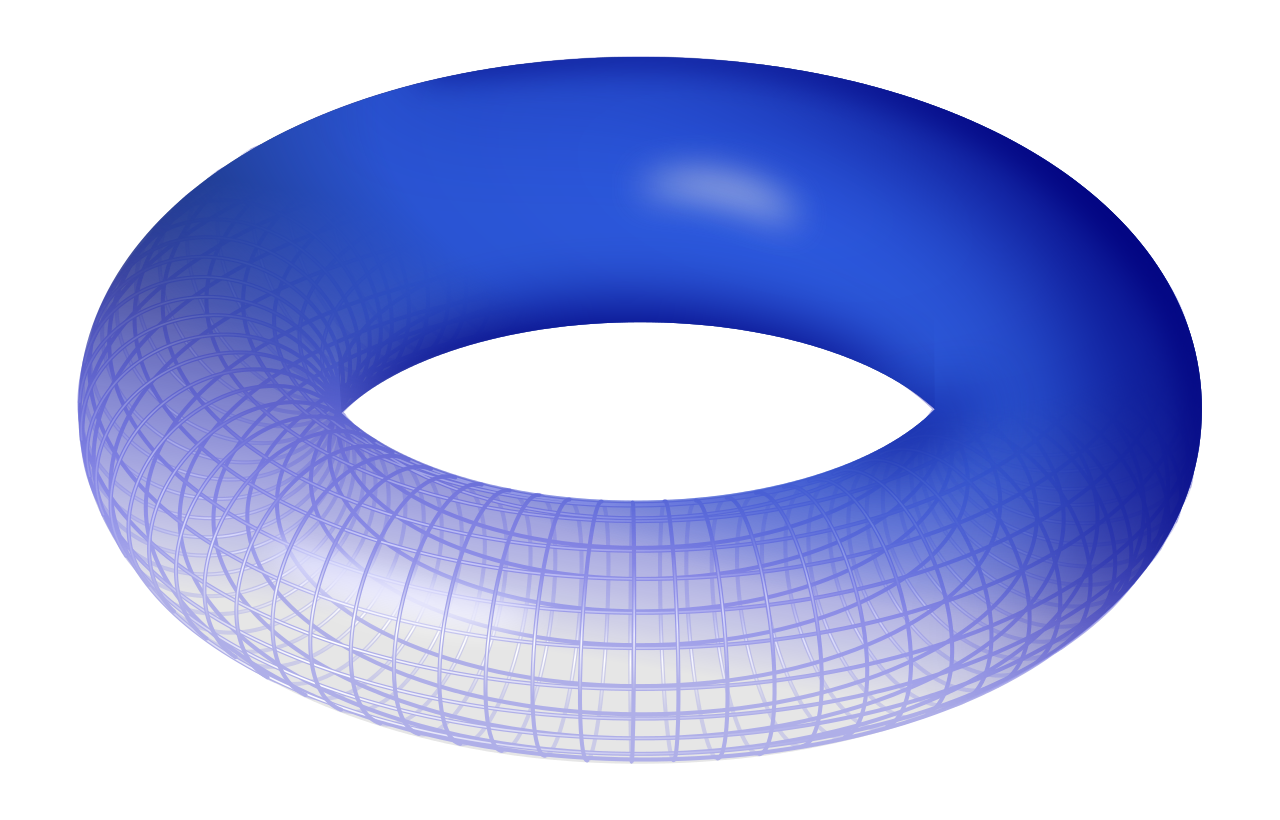
\includegraphics[width=0.5\linewidth]{images/Torus.png}
\caption{Representación clásica de un toro. Imagen extraída de \cite{Wikipedia:Torus}.}
\end{figure}

La expresión paramétrica de un toro es
\begin{equation}
\begin{tabular}{c c l}
$x$ & $=$ & $r \cos u \cos t + R \cos t$, \\
$y$ & $=$ & $r \cos u \sin t + R \sin t$, \\
$z$ & $=$ & $r \sin u$.
\end{tabular}
\nonumber
\end{equation}

Si renombramos esta expresión como
\begin{equation}\label{Uhlir03-14}
c_u = \cos u, \hspace{0.5cm} c_t = \cos t, \hspace{0.5cm} s_u = \sin u \hspace{0.5cm} \text{y} \hspace{0.5cm} s_t = \sin t,
\end{equation}
podemos representar la expresión paramétrica inicial en polinomios como
\begin{equation}\label{Uhlir03-15}
\begin{tabular}{r c c}
$x - r c_u c_t - R c_t$ & $=$ & $0$, \\
$y - r c_u s_t - R s_t$ & $=$ & $0$, \\
$z - r s_u$ & $=$ & $0$.
\end{tabular}
\end{equation}
Añadiendo las identidades
\begin{equation}
\begin{tabular}{r c c}
$c_u^2 + s_u^2 - 1 = 0$ & $=$ & $0$, \\
$c_t^2 + s_t^2 - 1 = 0$ & $=$ & $0$.
\end{tabular}
\end{equation}
La base de Gröbner reducida para el ideal $I$, generado por los polinomios (\ref{Uhlir03-14}) y (\ref{Uhlir03-15}), contiene 9 elementos. Uno solo de estos elementos no contiene variables en $c_u, s_u, c_t \text{ ó } s_t$, y tiene la forma
$$(x^2 + y^2 + z^2 - r^2 - R^2)^2 = 4 R^2 (z^2 - r^2),$$
la cual es la expresión implícita del toro.

\subsection{Método de la resultante}

El término { \em resultante} se suele introducir si se presenta la siguiente cuestión: ¿Cuándo dos polinomios en el anillo de polinomios $K[x]$ tienen un divisor común? Los métodos que usan la evaluación de la resultante se pueden usar para eliminar un subconjunto de variables del sistema inicial de ecuaciones algebraicas no lineales.
Un dato interesante de la resultante para polinomios en varias variables es que para $n+1$ polinomios ésta elimina $n$ variables a la par. A diferencia del método de la base de Gröbner, este método es no secuencial. La idea básica que subyace en las resultantes multidimensionales es la conversión de un problema de eliminación no lineal en uno lineal, lo cual ayuda a aplicar métodos conocidos de Álgebra Lineal para resolver el sistema.

Existen distintos tipos de resultante. La definición básica involucra dos polinomios en una variable, por ejemplo la resultante de Sylvester o Bézout, y a partir de ahí se puede ir generalizando a dos polinomios en dos variables y después a tres polinomios en dos variables, la resultante de Dixon. Esta última puede generalizarse a $n+1$ polinomios en $n$ variables. Aquí daremos una simple pincelada para dar la idea de las resultantes ya nombradas. Podemos encontrar más información en \cite{Berchtold00}.

\subsubsection*{Resultante de Sylvester}

El principal problema es la tendencia a encontrar si dos polinomios $f, g \in K[x]$ tienen divisor común. Existen varias maneras de encontrarlo, por ejemplo, el algoritmo de Euclides se puede usar para descomponer los polinomios en productos de factores simples. O por ejemplo, el siguiente lema.

\begin{lemma}
	Sean $f,g \in K[x]$ tales que $deg(f) = n > 0$ y $deg(g) = m > 0$. Se tiene que $f$ y $g$ tienen un divisor común si y sólo si existen polinomios $A, B \in K[x]$ verificando que
	\begin{enumerate}
		\item ambos polinomios $A$ y $B$ son no nulos,
		\item $A$ y $B$ tienen como mínimo grado $m-1$ y $n-1$ respectivamente y
		\item $Af + Bg = 0$.
	\end{enumerate}
\end{lemma}

\begin{definition}
	Sean $f, g \in K[x]$ dados como $f = a_n x^n + \dots + a_0$ y $g = b_m x^m + \dots + b_0$ donde $a_n, b_m \neq 0$, entonces la resultante de Sylvester de $f$ y $g$ es de la forma
$$\operatorname{Res}(f,g) = \operatorname{Det}(\operatorname{Syl}(f,g)).$$
Donde $\operatorname{Syl}(f,g)$ denota
	$$\begin{pmatrix}
	a_n & & & & & b_m & & & & \\
	a_{n-1} & a_n & & & & b_{m-1} & b_m & & & \\
	a_{n-2} & a_{n-1} & a_n & & & b_{m-2} & b_{m-1} & b_m & & \\
	\vdots & \vdots & & \ddots & \vdots & \vdots & \vdots & \vdots & \ddots & \\
	a_1 & \dotso & \dotso & \dotso & a_{n} & b_1 & \dotso & \dotso & \dotso & b_{m} \\
	a_0 & \dotso & \dotso & \dotso & a_{n-1} & b_0 & \dotso & \dotso & \dotso & b_{m-1} \\
	 & a_0 & \dotso & \dotso & a_{n-2} & & b_0 & \dotso & \dotso & b_{m-2} \\
	 & & \ddots & \vdots & \vdots & & & \ddots & \vdots & \vdots \\
	 & & & a_1 & a_0 & & & & b_1 & b_0 \\
	 & & & & a_0 & & & & & b_0
	\end{pmatrix}$$
y los espacios en blanco de la matriz denotan ceros.
\end{definition}

Ahora realizaremos un ejemplo sencillo para comparar este método con el de la base de Gröbner.

Sean por ejemplo los polinomios:
$$f = x^2 y - 1, \hspace{2cm} g = x^2 + y^2 + xy - 4.$$

Aplicando el método de la resultante de Sylvester tenemos
$$\operatorname{Res}(f,g) = \operatorname{Det} \begin{pmatrix}
y & 0 & 1 & 0 \\
0 & y & y & 1 \\
-1 & 0 & y^2 - 4 & y \\
0 & -1 & 0 & y^2 - 4
\end{pmatrix} = y^6 - 8y^4 + y^3 + 16y^2 - 8y + 1.$$

Para comparar podemos ver la solución obtenida mediante el método de la base de Gröbner para el ideal $I = \langle f,g \rangle$ cuya base de Gröbner reducida respecto del orden lexicográfico sería
$$\langle x - 4y^5- y^4 + 32y^3 + 4y^2 - 64y + 16 , y^6 - 8y^4 + y^3 + 16y^2 - 8y + 1 \rangle.$$

\subsubsection*{Resultante de Bézout}

Es similar a la resultante de Sylvester, salvo que la definición de matriz de Bézout es un poco más dificultosa que ésta, pero a cambio ésta tiene dimensión $n \times n$ en lugar de la dimensión $(n+m) \times (n+m)$. En consecuencia, la evaluación del determinante de la matriz Bézout es mucho más rápido.

\subsubsection*{Resultante de Dixon}

Es una versión generalizada de la resultante y matriz de Bézout para tres polinomios en dos variables. Entonces la resultante de Dixon se generaliza para $n+1$ polinomios en $n$ variables.

\subsection{El método de Wu-Ritt}

En esta sección daremos una breve introducción a la teoría de este método. Éste se basa en la aproximación de Wu-Ritt para encontrar un conjunto característico para un sistema de ecuaciones no lineales. Dado un sistema de ecuaciones polinomiales $S = \{ f_1, \dotso, f_m \}$ se transforma en una forma triangular $S'$. Es importante notar que si el número $n$ de variables es mayor que el número de ecuaciones del conjunto $S$, entonces el conjunto de variables se divide en dos subconjuntos: las variables independientes, que denotaremos por $\{ u_1, \dotso, u_k \}$, y las dependientes, que denotaremos por $\{ y_1, \dotso, y_l \}$.

La pseudodivisión de polinomios de varias variables es la operación clave en la computación de conjuntos característicos. Para realizar la pseudodivisión se da uso de la representación recursiva de los polinomios con lo cual se define la siguiente reducción polinomial.

Un polinomio $f_i$ se reduce respecto de otro polinomio $f_j$ si verifican una de las dos siguientes condiciones:
\begin{enumerate}
\item La mayor variable de $f_i$ es menor, con respecto a $\prec$ , que la mayor variable de $f_j$.
\item El grado de la mayor variable en $f_j$ es mayor que el grado de la mayor variable en $f_i$.
\end{enumerate} 

Si $f_i$ no es reducible respecto de $f_j$, entonces $f_i$ se reduce a $r$ mediante la pseudodivisión entre $f_j$.

\begin{definition}
	Dado un conjunto finito $\Sigma$ de polinomios $u_1, \dotso, u_k, y_1, \dotso, y_l$ un conjunto característico $\Phi$ de $\Sigma$ se define de cualquiera de las siguientes maneras:
	\begin{enumerate}
		\item $\{ g_1 \}$ donde $g_1$ es un polinomio de $\{ u_1, \dotso, u_k \}$.
		\item Una cadena $\langle g_1, \dotso, g_l \rangle$ donde cada $g_i$ es un polinomio en $\{ u_1, \dotso, u_k, y_1, \dotso, y_i \}$, con coeficiente líder $LC(g_i)$, tales que:
		\begin{itemize}
			\item Cualquier cero de $\Sigma$ es un cero de $\Phi$.
			\item Cualquier cero de $\Phi$ que no es cero de ninguno de los coeficientes líderes $LC(g_i)$ es un cero de $\Sigma$.
		\end{itemize}
	\end{enumerate}
\end{definition}
Podemos encontrar más información sobre el presente método en \cite{Berchtold00}, \cite{Gallo91_2} o \cite{Gallo91_1}.

\section{Conclusiones}

Todos los métodos mencionados tienen una característica común: si hacemos uso de ellos para convertir la expresión paramétrica de un objeto a la expresión implícita de éste entonces lo que obtenemos es una sola ecuación. A partir de ahí las superficies pueden ser visualizadas con métodos de visualización directa.

Por supuesto, esto es solo un tipo de métodos de implicitación de superficies, ya que existe una  gran variedad. Alguno ya ha sido mencionado al comienzo de este capítulo y otros pueden ser consultados en la bibliografía. En este tipo de métodos no es necesario conocer la expresión paramétrica del objeto.
\chapter{Representación y visualización de superficies implícitas}

Escribir introducción.

\section{Representación de superficies algebraicas y blobs}

\subsection{Superficies algebraicas}

Una superficie se dice algebraica si se define por polinomios cuyo grado indica el grado de la superficie. El grado indica el número de intersecciones de la superficie y una recta.\cite{Bloomenthal97} Por ejemplo un plano tiene grado 1 mientras que una esfera tiene grado 2. El uso de polinomios tiene la ventaja de ser menos costoso, en tiempo de renderización, que cualquier otra representación analítica general.
\par Las superficies algebraicas más comunes son las cuadráticas. Este tipo de superficies son fáciles de renderizar son muy pocos parámetros para controlar su forma, además, es posible usar coordinadas homogéneas para aplicar transformaciones afines. A continuación mostramos típicas superficies cuadráticas como son la esfera, el cilindro y el cono.

\begin{figure}[h]
	\centering
	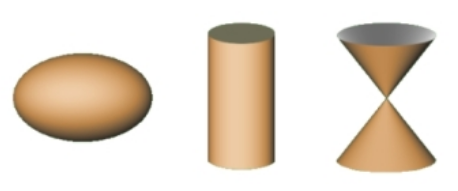
\includegraphics[scale=0.7]{images/florez4.png}
	\caption{Ejemplos básicos de superficies cuadráticas.}
\end{figure}

\subsection{Blobs}

Los blobs son sumas de distribuciones gaussianas inspiradas en la distribución de densidad de las moléculas. Este tipo de superficies fueron usadas por primera vez por Blinn \cite{Blinn82} para renderizar una animación del ADN para el programa de televisión Cosmos de Carl Sagan en donde cada átomo era aproximado por una esfera gaussiana.
\par La suma de esferas gaussianas genera una unión entre las superficies. Blinn propuso la función

\begin{equation}
f(x,y,z) = \sum_{i=1}^{n} b_i e^{-a_i r_i^2} - 1
\nonumber
\end{equation}

donde cada función está centrada en un término $r$. El término $r$ se calcula como $r(x,y,z) = \sqrt{(x - x_i)^2 + (y-y_i)^2 + (z-z_i)^2}$. El término $b$ representa la altura de la función y el término $a$ es la desviación estándar. El efecto de la función blob se puede modificar cambiando los parámetros.

\begin{figure}[h]
	\centering
	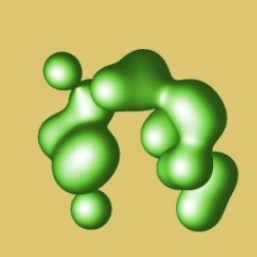
\includegraphics[scale=0.7]{images/florez3.png}
	\caption{Ejemplo de sumas de esferas gaussianas.}
\end{figure}

La función exponencial define una esfera gaussiana que tiende a infinito a la par que la exponencial tiende a cero. Esto significa que cada esfera gaussiana influye sibre las demás sin importar la separación que exista entre ellas. Los objetos flexibles\cite{Wyvill86} computan als esferas usando aproximaciones polinomiales.

\section{Métodos de visualización}

En esta sección cubrimos dos de los métodos de visualización usados y referenciados en la bibliografía de superficies implícitas de forma más frecuente: Poligonalización y ray tracing. Cubriremos ambos con detalle, pero cabe destacar que en el resto del Trabajo Fin de Máster nos centraremos en el desarrollo del segundo.

\subsection{Poligonalización de superficies implícitas}

La idea general de los métodos de poligonalización consiste en la creación de polígonos que representen la superficie implícita. Los polígonos son fáciles de renderizar en los sistemas gráficos modernos, por tanto, este método suele ser el elegido cuando necesitamos de visualización interactiva.
\par Existen varios métodos  de poligonalización de superficies, siendo los más populares:

\begin{itemize}
	\item El llamado{ \em método de las celdas fijas}\cite{Bloomenthal90} consistente en dividir el espacio en poliedros de forma conveniente (cubos, tetraedros,...) y, tras esto, en calcular la intersección de la superficie con  las aristas de los poliedros para así definir los vértices de la poligonalización. Estos vértices han de ordenarse para crear poígonos convexos.
	\par Obviamente la calidad del resultado depende en gran medida de como de { \em fina} sea la división del espacio, esto es, si los poliedros son demasiado grandes entonces se perderan una gran cantidad de detalles y si son demasiado pequeños crearán polígono en exceso que realentizarán la renderización.
	\par Este problema se puede solucionar con una serie de métodos adaptativos donde el tamaño de la celda según el detalle de la superficie, véase, si en una zona nos interesa hacer una poligonalización más detallada allí habrá una división más fina. Aunque estos métodos son difíciles de implementar y aún no son muy populares por esta razón y las celdas de tamaño fijo suelen ser la opción más común.
	\item El segundo método más común son los{ \em marching methods} que consisten en crear, de forma sucesiva, un mallado triangular comenzando con un punto o un polígono dado. Este método lo explicaremos mejor a continuación con un ejemplo claro donde explicaremos un algoritmo concreto extraído de \cite{Hartmann03}.
\end{itemize}

\begin{remark}
	El siguiente algoritmo está extraído de \cite{Hartmann03}, pero al aparecer en \cite{Hartmann98} los derechos pertenecen a Springer-Verlag.
\end{remark}

\subsection{El algoritmo de triangulación}

La formulación del algoritmo de triangulación no usa ninguna representación especial de la superficie para ser triangulada. Las operaciones dependientes de la representación están implícitamente en el apartado de \texttt{surfacepoint} que se define a continuación.
\par El próximo apartado nos presenta las ideas básicas del algoritmo. Después el procedimiento \texttt{surfacepoint} y la estructura de los datos usados es introducida. Finalmente se explican los pasos del algoritmo en detalle.

\subsubsection{La idea del algoritmo}

\begin{enumerate}
	\item[S0] Escoge un punto $s$ cercano a la superficie. Determina el correspondiente punto $p_1$ de la superficie. Rodea $p_1$ de un hexágono regular $q_2, \dotso, q_7$ en el plano tangente. Con el procedimiento \texttt{surfacepoint} determina los puntos $p_2, \dotso, p_7$ correspondientes a los  puntos iniciales $q_2, \dotso, q_7$.
	\par Ya hemos construido los primeros seis triángulos de la triangulación.
	\par Entonces al conjunto ordenado de puntos $p_2, \dotso, p_7$ lo llamaremos{ \em polígono delantero actual} $\Pi_0$. Si la triangulación se puede limitar por curvas cerradas $\Gamma_1, \\Gamma_2,\dotso$ podemos determinar los polígonos delanteros $\Pi_1, \Pi_2, \dotso$ ligados a las curvas.
	
\begin{figure}[h]
	\centering
	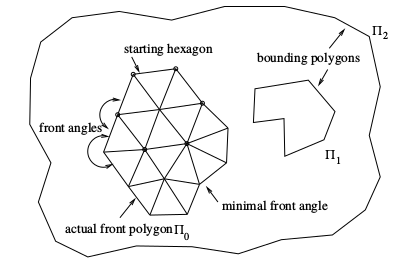
\includegraphics[scale=0.7]{images/hartmann1.png}
	\caption{Nociones básicas del algoritmo de triangulación.}
\end{figure}	
	
	\item[S1] Para cada punto del polígono $\Pi_0$ determinamos el ángulo del área aún por triangular. A estos ángulos los llamamos{ \em ángulos delanteros}.
	
	\begin{figure}[h]
		\centering
		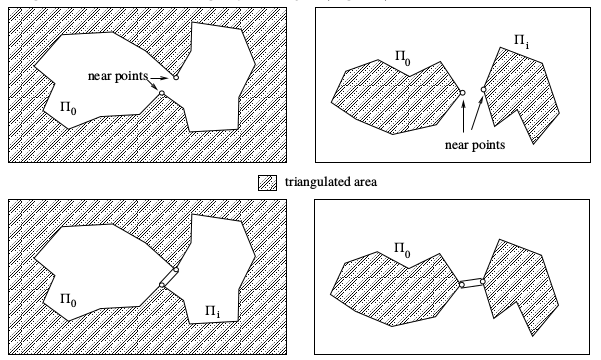
\includegraphics[scale=0.5]{images/hartmann2.png}
		\caption{Dividiendo y uniendo el polígono $\Pi_0$.}
	\end{figure}
	
	\item[S2] Revisamos si algún punto $p_i$ de $\Pi_0$ está cerca. Con cerca entendemos:
	\begin{itemize}
	\item Un punto de $\Pi_0$  distinto de $p_i$ y de su entorno.
	\item Un punto de cualquier otro polígono $\Pi_k$ distinto.
	\end{itemize}
	En el primer caso dividimos el polígono $\Pi_0$ en dos nuevos polígonos $\Pi_0$ y $\Pi_1$. En el segundo caso unimos los dos polígonos en uno nuevo al que llamaremos $\Pi_0$ y será nuestro nuevo polígono delantero actual.
	\item[S3] Determinar un punto $p_m$ del polinomio $\Pi_0$ con un ángulo delantero mínimo. Rodea $p_m$ por triángulos con ángulos cercanos a $\frac{\pi}{6}$. ELimina $p_m$ del polígono $\Pi_0$ e inserta los nuevos puntos en $\Pi_0$.
	\item[S4] Repite los pasos 1, 2 y 3 hasta que $\Pi_0$ consista sólo en tres puntos que generan un nuevo triángulo. Si aún queda algún polígono restante se convierte en el nuevo $\Pi_0$ y se repiten los pasos 1, 2 y 3. Una vez ya no queden más polígonos, habremos terminado y la triangulación estará completada.
\end{enumerate}

\subsubsection{El procedimiento \texttt{surfacepoint}}

Un paso fundamental del algoritmo es determinar el punto $p$ de la superficie que está cerca de un punto $q$ en un entorno de la superficie. El vector $q - p$ no ha de ser necesariamente perpenticular a la superficie. Debido a que casi todas las superficies pueden ser numéricamente implicitadas, daremos a solución para superficies implicitas.
\par Comenzamos con una superficie implícita $\Phi$ definida por una función $f(x) = 0$ para la cual su gradiente $\nabla f$ existe y no se anula para ningún punto de la superficie y un punto $q$ en un entorno de la superficie.
\par El siguiente procedimiento calcula un punto de la superficie $p$, un normal y dos vectores tangentes al punto $p$.

\begin{enumerate}
	\item \begin{itemize}
		\item $u_0 := q$
		\item Repetir $u_{k+1} := u_k - \frac{f(u_k)}{\nabla f(u_k)^2} \nabla f(u_k)$ hasta que $\| u_{k+1} - u_k \|$ es sficientemente pequeño.
		\item $p := u_{k+1}$ 
\end{itemize}		
	\item Definimos el normal a la superficie en $p$ como $n := \frac{\nabla f(p)}{\| \nabla f(p) \|}$.
	\item Para los vectores tangentes: \begin{itemize}
		\item $t_1 := \frac{1}{\| \sqrt{n_x^2 + n_y^2} \|} (n_y, -n_x, 0)$ si $n_x > 0.5$ ó $n_y > 0.5$.
		\item En otro caso elegimos $t_1 := \frac{1}{\| \sqrt{n_x^2 + n_z^2} \|} (-n_z, 0, n_x)$.
		\item $t_2 := n \times t_1$
	\end{itemize}
\end{enumerate}

\subsubsection{La estructura}

Para la construcción de los triángulos necesitamos un paso de longitud $\delta_t > 0$ qie es aproximadamente la longitud de las aristas.
\par Para cada putno $p_i$ guardamos la siguiente información:
\begin{itemize}
	\item Las coordinadas.
	\item El normal y los tangentes a la superficie en $p_i$ tales que son ortonormales entre sí.
	\item El ángulo delantero de $p_i$ si es un punto delantero de $\Pi_0$.
	\item La variable booleana \texttt{angle\_changed} con \texttt{angle\_changed = true} si el ángulo delantero cambió y tiene que ser recalculado.
	\item La variable booleana \texttt{border\_point}, con el valor \texttt{true} si el punto $p_i$ es en el borde de la triangulación y debería ser ignorado para futuros cálculos.
\end{itemize}

Los triángulos serán numerados de forma consecutiva. Para cada triángulo guardaremos el valor numérico de sus vértices.

\subsubsection{S0}

Sea $s$ un punto inicial en un entorno de la superficie. Entonces \texttt{surfacepoint} nos determina el primer punto $p_1$ de la triangulación y el sistema ortonormal $n_1, t_{11} \text{ y } t_{12}$. El resto de puntos $P_2, \dotso, p_7$ son el resultado de aplicar \texttt{surfacepoint} a:

$$q_{i+2} = p_1 + \delta_t cos\left(\frac{i \pi}{3}\right)t_{11} + \delta_t sen\left(\frac{i\pi}{3}\right)t_{12} \hspace{1cm} i = 0, \dotso, 5$$

Ya hemos obtenido los primeros seis triángulos.

\subsubsection{S1}

Si un punto $p_{0i}$ del polígono delantero $\Pi_0 = (p_{01}, \dotso, p_{0N_0})$ acaba de ser incluido o un punto cercano a $p_{0i}$ es un nuevo punto, entonceces es necesario recalcular elángulo delantero $\omega$ del punto $p_{0i}$. Sea:

\begin{itemize}
	\item $v_1 := p_{0,i-1}$ si $i>1$ ó $v_1 := p_{0N_0}$ si $i=1$.
	\item $v_2 := p_{0,i+1}$ si $i<N_0$ ó $v_2 := p_{01}$ si $i=N_0$.
	\item $(\xi_1,\eta_1,\zeta_1)$ y$(\xi_2,\eta_2,\zeta_2)$ las coordenadas de $v_1$ y $v_2$, respectivamente, en el sistema local ortonormal $n, t_1$ y $t_2$ en el punto $p_{0i}$.
	\item $\omega_i$ el ángulo polar de $(\xi_i, \eta_i)$. 
\end{itemize}

Entonces el ángulo delantero en el punto $p_{0i}$ es $\omega = \omega_2 - \omega_1$ si $\omega_2 \geq \omega_1$ ó $\omega = \omega_2 - \omega_1 + 2\pi$ en caso contrario.

\subsubsection{S2}

Para prevenir el solapamiento de nuevos triaángulos sobre los ya existentes comprobaremos:

\begin{itemize}
\item Las distancias dos a dos de los puntos que componen $\Pi_0$. Si hay puntos $p_{0i}$ y $p_{0j}$, con $i<j$, que no son vecinos, ni vecinos de vecino y $\| p_{0i} - p_{0j} \| < \delta_t$ entonces $\Pi_0$ se separa en dos polígonos.
\item Las distancias de puntos de $\Pi_0$ a puntos del resto de polígonos $\Pi_k$. Si hay puntos $p_{0i} \in \Pi_0$ y $p_{mj} \in \Pi_m$ tales que $\| p_{0i} - p_{mj} \| < \delta_t$, entonces los polígonos $\Pi_0$ y $\Pi_m$ se unen.
\end{itemize}

\begin{figure}[h]
\centering
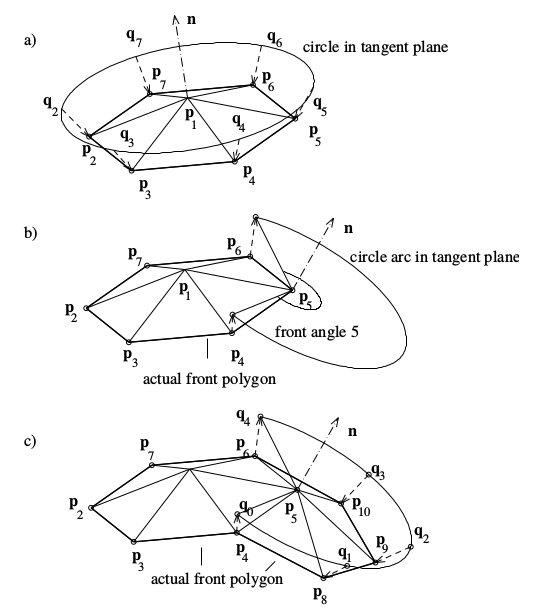
\includegraphics[scale=0.6]{images/hartmann3.png}
\caption{Los primeros pasos del algoritmo.}
\end{figure}

\subsubsection{S3}

Sea $p_{0m}$ un punto de $\Pi_0$  con un ángulo delantero mínimo $\omega$. Completamos la triangulación en $p_{0m}$ de la siguiente manera:

\begin{figure}[h]
\centering
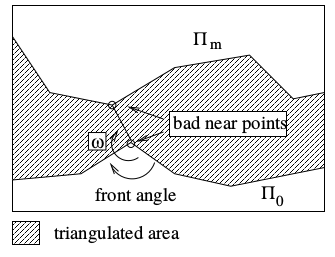
\includegraphics[scale=0.5]{images/hartmann4.png}
\caption{Puntos cercanos \textit{malos} y su detección.}
\end{figure}

\begin{enumerate}
\item Determinamos los vecinos $v_1$ y $v_2$ de $p_{0m}$.
\item Determinamos el número $n_t$ de triángulos que van a ser generados:
$$n_t := \mathtt{trunc}\left( \frac{3\omega}{\pi} \right) + 1 \hspace{1cm} \Delta \omega := \frac{\omega}{n_t}$$
Corrección de $\Delta \omega$ para casos extremos:
\begin{itemize}
\item Si $\Delta \omega < 0.8$ y $n_t > 1$ entonces $n_t \to n_t - 1$ y $\Delta \omega = \frac{\omega}{n_t}$.
\item Si $\Delta \omega < 0.8$, $n_t = 1$ y $\| v_1 - v_2 \| > \frac{5}{4} \delta_t$ entonces $n_t = 2$ y $\Delta \omega \to \frac{\Delta \omega}{2}$.
\item Si $\omega < 3$ y $\| v_1 - p_{0m} \| \leq \frac{1}{2} \delta_t$ (ó $\| v_1 - p_{0m} \| \leq \frac{1}{2} \delta_t$) entonces $n_t = 1$.
\end{itemize}

\begin{figure}[h]
\centering
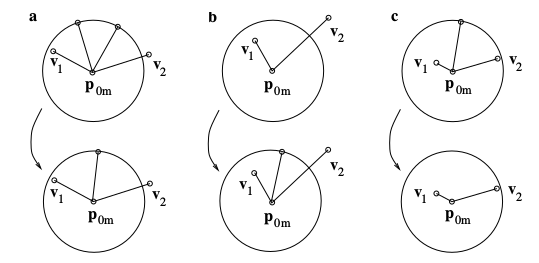
\includegraphics[scale=0.5]{images/hartmann5.png}
\caption{Correcciones de los casos extremos.}
\end{figure}

\item Generamos los triángulos:
\par Si $n_t = 1$ entonces tenemos un nuevo triángulo $(v_1, v_2, p_{0m})$ en otro caso sean $q_0$ y $q_{n_t}$ las proyecciones ortogonales de $v_1$ y $v_2$ en el plano tangente en el punto $p_{0m}$ y sea $q_i$ el resultado de una rotación de ángulo $i \Delta \omega$ alrededor del normal a la superficie en $p_{0m}$ aplicada a $p_{0m} + \delta_t \frac{q_0 - p_{0m}}{\| q_0 - p_{0m} \|}$. Aplicando el procedimiento \texttt{surfacepoint} a $q_i$ obtendremos nuevo puntos $p_{N+i}$ $i = 1, \dotso, n_t -1$, donde $N$ es el total de puntos existentes hasta el momento, y $n_t$ nuevos triángulos.
\item Renovamos el polígono $\Pi_0$:
\par Borramos el punto $p_{0m}$ y, si $n_t > 1$, insertamos en su posición los nuevos puntos $p_{N+1}, \dotso, p_{N+n_t-1}$. Todas las variables booleanas tiene el valor \texttt{true} para asegurarnos de que los nuevos cálculos se realizan.
\end{enumerate}

\subsubsection{Ejemplos de superficies trianguladas}

\textbf{Esfera}
\[\]
Triangulación de la esfera $x^2 + y^2 + z^2 - 4 = 0$ comenzando por el punto $(1,1,1)$ y paso de longitud $\delta_t = 0.3$. La siguiente imagen muestra los primeros cuatro polígonos delanteros y la situación tras 101 y 1531 triángulos. La triangulación total involucra 1534 triángulos.
\[\]
\begin{figure}[h]
\centering
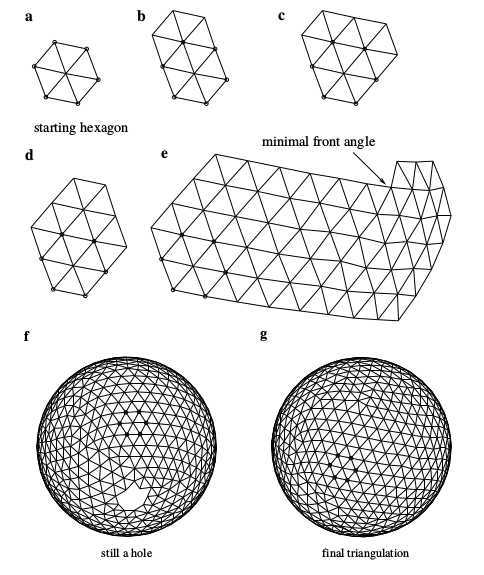
\includegraphics[scale=0.7]{images/hartmann6.png}
\caption{Proceso de triangulación de la esfera.}
\end{figure}

\newpage
\textbf{Cilindro}
\[\]
Triangulación del cilindro $x^2 + y^2 - 1 = 0$ comenzando por el punto $(1,0,0)$ y paso de longitud $\delta_t = 0.2$. 
\[\]
\begin{figure}[h]
\centering
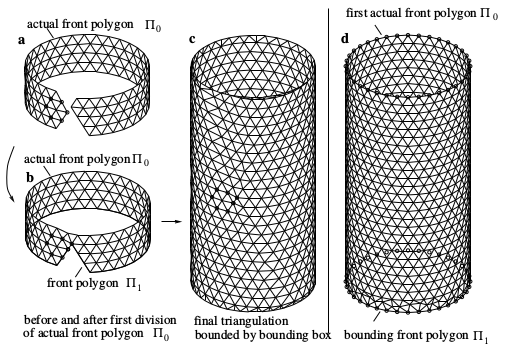
\includegraphics[scale=0.8]{images/hartmann7.png}
\caption{Proceso de triangulación del cilindro.}
\end{figure}

\newpage
\textbf{Toro}
\[\]
Triangulación del cilindro $(x^2+y^2+z^2+0.8775) - 4(x^2+y^2)=0$ comenzando por el punto $(1,0,0.5)$ y paso de longitud $\delta_t = 0.1$.
\[\]

\begin{figure}[h]
\centering
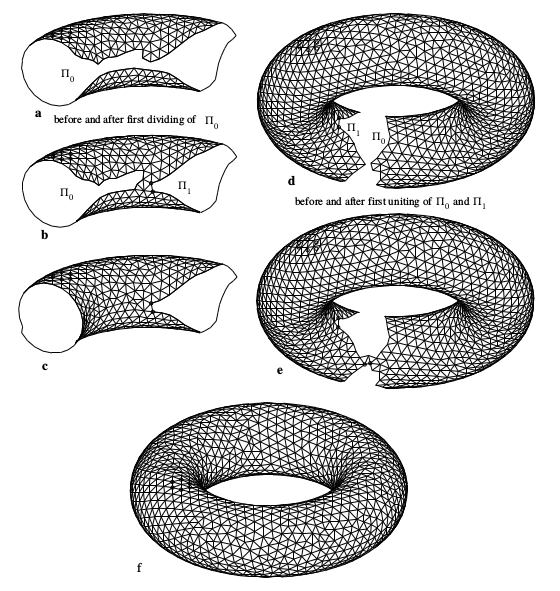
\includegraphics[scale=0.7]{images/hartmann8.png}
\caption{Proceso de triangulación del toro.}
\end{figure}

\newpage
\subsection{Ray Tracing en superficies implícitas}

En 1980, Whitted\cite{Whitted80} propuso un método dpara generar imágenes de alta calidad usando modelos geométricos básicos. Este método evolucionó en lo que hoy se conoce como Ray Tracing, donde la interacción entre rayos de luz y objetos en la nauraleza es simulado: la luz, ya sea artificial o natural, rebota con los objetos y esto es lo que llega a nuestros ojos e interpretamos las propiedades de los objetos, véase color, transparencia, brillo... Además la luz indirecta puede rebotar en varios objetos antes de llegar a nuestros ojos.

\begin{figure}[h]
\centering
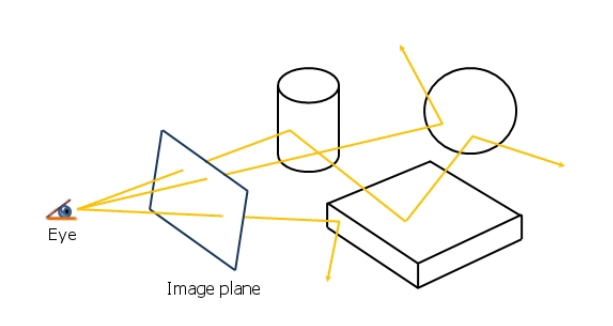
\includegraphics[scale=0.5]{images/florez1.png}
\caption{Rayos de luz rebotando en distintos objetos antes de llegar a nuestros ojos. El plano imagen en la figura se ve cruzado por los rayos; este plano puede contener una representación bidimensional de la escena tridimensional.}
\end{figure}

Usando esta técnica de renderización es posible obtener una representación realista de  de distintos tipos de escenas.
\par En la naturaleza la luz proviene de las llamadas fuentes de luz y, tras rebotar en los objetos del medio, algunos de los rayos llegan a nuestros ojos. Por tanto, analizando el problema, podemos darnos cuenta que, computacionalmente hablando, es muy costoso intentar simular todos los rayos provenientes del foco de luz basándonos en que muchos de los rayos nunca llegarán a nuestro ojo. Por esa razón  es mejor modelar el proceso inverso, esto es, trazar los rayos desde el ojo y buscar las intersecciones con  los objetos del medio.

\subsection{El algoritmo de Ray Tracing}

El método del Ray Tracing es de los llamados{ \em píxel a píxel}. Uno o más rayos de luz son trazados en cada uno de los píxeles en un plano imagen o pantalla. El objetivo es encontrar las intersecciones con los objetos del medio conforme vayamos realizando el trazado de los rayos. Generalmente se suele buscar la primera intersección ya que, en caso de haber más de una, suelen estar obstruidas por el propio objeto.

En la figura \ref{florez27} introducimos el proceso de construcción de un rayo. El punto $c$ representa el origen. Un rayo que comienza en este punto se envía a travez de un píxel en la pantalla con dirección $\vec{cs}$. Estos rayos tienen coordenadas con respecto al sistema $uvw$, mientras que el objeto tiene su propio sistema de referencia $xyz$. Esta independencia de los sistemas de referencia permite ver la escena desde cualquier posición arbitraria.

\begin{figure}[h]
\centering
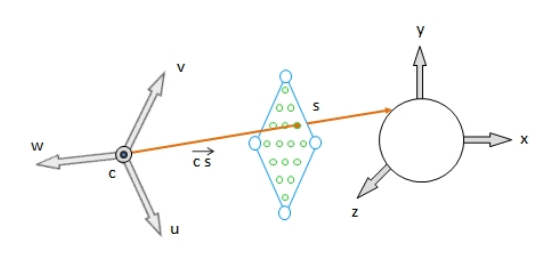
\includegraphics[scale=0.5]{images/florez2.png}
\caption{Definición de un rayo cruzando una pantalla. Si el rayo interseca alguna superficie, el color se calcula y asignado al píxel en la pantalla.}
\label{florez27}
\end{figure}

Si hay alguna intersección entre el rayo y el objeto el color es calculando tomando en cuenta la dirección del vector normal del punto de intersección y la posición de las luces. La aportación de las luces indirectas también se calcula. La suma de todas las posibles aportaciones se usa para asignar el color correspondiente en el píxel.
\[\]
\textbf{Análisis de la intersección}
\[\]
Un rayo se define como:
\begin{equation}
\begin{split}
x = c_x + t(x_s - c_x) \\
y = c_y + t(y_s - c_y) \\
z = c_z + t(y_z - c_z)
\end{split}
\nonumber
\end{equation}

Donde $(c_x,c_y,c_z)$ es origen o punto de vista, $(x_s,y_s,z_s)$ es el punto donde el rayo cruza la pantalla y $t$ es el parámetro del rayo.
\par La intersección entre la superfície implícita $f(x,y,z) = 0$ y el rayo viene definida por la ecuación:

$$g(t) = 0$$

donde $g(t)$ es la función $g : \mathbb{R}_0 \to \mathbb{R}^3$ definida por:

\begin{equation}
g(t) \equiv f(c_x + t(x_s - c_x), c_y + t(y_s - c_y), c_z + t(y_z - c_z))
\nonumber
\end{equation}
De este modo, el problema se reduce a encontrar las raíces de la función $g$.
\par Estas soluciones se sustituyen en la definición parametrica del rayo para encontrar el punto de intersección y el valor del vector normal.
\par Existen muchas maneras  de encontrar las raíces de $g$. Las manera más clásicas son el método de la bisección o de Newton\cite{Hart01}. También existen de otro tipo como: técnicas fuzzy,\cite{Foufou96} aritmética de intervalos\cite{Mitchell90} o constantes de Lipschitz.\cite{Kalra89}

\subsection{Ray Tracing eficiente}

Como ya hemos comentado el principal problema del algoritmo de Ray Tracing es la falta de eficiencia. Muchos autores han propuesto diferentes técnicas de mejora de la eficiencia pero se pueden clasificar en tres grupos:

\begin{itemize}
\item Intersecciones más rápidas.
\item Trazar menor cantidad de rayos.
\item Generalización de los rayos.
\end{itemize}

La técnica más básica para acelerar el Ray Tracing es el llamado{ \em volumen delimitador o límite},que consiste en crear un volumen que contenga a nuestro objeto y que el cálculo de la intersección de los rayos con éste sea menos costoso que con el objeto en sí. La primera propuesta de volumen delimitador fue la esfera\cite{Whitted80} por la simplicidad y por la facilidad para probar la intersección de los rayos con ésta. La idea es recubrir coda objeto con una esfera, si un rayo interseca a una esfera, entonces se analiza el caso dentro de la esfera, en caso contrario no es necesario. Si además añadimos lo que se suele llamar{ \em jerarquía} el orden del algoritmo se puede reducir a $log(n)$.
\par Otra técnica bastante común en la literatura especializada es la subdivisión del espacio en la cual el espacio que rodea a nuestro objeto se divide y se descartan las subdivisiones que no contienen parte del objeto alguno. Podemos dividir el espacio de manera regular o de manera adaptativa como con la poligonalización, pero conlleva los mismos inconvenientes.\\ La ventaja que  tiene este método es que, al ordenar las divisiones, sólo hay que probar el rayo para cada una de éstas en lugar de para el espacio completo para buscar la primera intersección.
\par Ya como final tenemos las llamadas técnicas direccionales en la que se mejora la técnica anterior discretizando también las direcciones.

\section{Conclusiones}

En este capítulo hemos visto distintas maneras de representar y visualizar superficies expresadas de forma implícita, de las cuales ya hemos nombrado sus ventajas e inconvenientes. En términos de coste computacional y velocidad de renderización éstas no presentan ningún reto y presentan una serie de propiedades que las hacen muy atractivas.
\par En el siguiente capítulo haremos una introducción al Análisis de Intervalos para mejorar la capacidad de computación y tratar de solventar los problemas de redondeo de las máquinas debido a los puntos flotantes.
\chapter{Análisis de intervalos}

El Análisis de Intervalos es una rama de las Matemáticas que lidia con los problemas de redondeo debido al uso de la aritmética de coma flotante. Los ordenadores tienen registros de coma flotante para representar los números reales. Como es bien sabido, hay números reales que no tienen representación finita, por esa razón estos números tienen que ser redondeados.
\\Este tipo de situación crea problemas de imprecisión numérica que se puede propagar y acumular a los largo de los algoritmos, en especial en aquellos que son recursivos.
\\Aunque es posible trabajar con un gran tamaño de bits para representar a los números, este conjunto de números es, de hecho, una representación digital que, obviamente, no tiene las mismas propiedades que el conjunto de números reales.
\\Un ejemplo muy básico puede mostrarnos este problema:
\begin{itemize}
	\item a = \texttt{random()}
	\item b = \texttt{random()}
	\item c = a + b
	\item c = c - a - b
\end{itemize}

Por lógica de cómo trabajamos con el conjunto de números reales se esperaría que el valor final de $c$ sea cero, pero este puede no ser el caso dependiendo del programa de cálculo que tomemos en un ordenador convencional.

Hay una gran cantidad de áreas de investigación en las cuales en Análisis de Intervalos ha sido aplicado para mantener la precisión numérica: Ingeniería de control y supervisión, modelización geométrica y diseño por ordenador.
\\Aparte también hay una serie de{ \em catástrofes} documentadas que podrían haber sido evitadas usando Análisis de Intervalos. Por ejemplo:
\begin{itemize}
	\item Un misil Patriot falló debido a la acumulación de errores de redondeo.
	\item La explosión del Arianne 5 causada por un error de exceso.
\end{itemize}

En este capítulo presentaremos la nociones, operaciones y propiedades básicas del Análisis de Intervalos. Además también haremos una introducción al Análisis de Intervalos Modal que completa la definición clásica de Análisis de Intervalos.

\section{Planteamiento}

La computación numérica de problemas teóricos en un ordenador requiere que los números reales $\mathbb{R}$ sean representados con una cantidad limitada de cifras decimales. Por supuesto, es posible usar un conjunto de números suficientemente grande de números con una gran cantidad de cifras decimales, pero aún así habrá números reales que no podrán ser representados.
\\Esto significa que, cuando traducimos un problema teórico a un problema computacional, estamos trabajando con un conjunto de{ \em números digitales}, llámese $DI$, también conocidos como números en coma flotante.

Los números reales dan soporte a aquellos modelos donde las magnitudes continuas están presentes. Sin embargo, como sabemos, los ordenadores trabajan con truncamiento de números reales. Por tanto, es posible que parte de la información se pierda. Las operaciones deberían restringirse a un intervalo obtenido por medias de redondeo, lo que nos da una identificación operacional de los valores calculados.

Dados dos valores reales $\underline{a}$ y $\overline{a}$, un intervalo $A$ se define como
\begin{equation}
A = [\underline{a},\overline{a}] = \{ x \in \mathbb{R} : \underline{a} \leq x \leq \overline{a} \},
\nonumber
\end{equation}
donde $\underline{a}$ y $\overline{a}$ se conocen como el ínfimo y el supremo del intervalo respectivamente.

Para mantener la representación exacta del número, debemos realizar redondeo al número digital más próximo. Este redondeo es necesario para que la definición anterior sea válida. El uso del Análisis de Intervalos con números digitales nos proporciona un control automático de los errores de redondeo.

En la construcción de intervalos, denotados por $I(\mathbb{R})$, muchas de las propiedades de los números reales se pierden, véase la propiedad distributiva, y se obtienen otras como la relación de inclusión.
\\ Los ordenadores trabajan con el conjunto $DI$, por esa razón el conjunto de intervalos con base en $DI$, denotado por $I(DI)$, es el usado para las operaciones algorítmicas. Esto significa que, mientras $I(DI)$ admita operaciones sobre el conjunto $DI$ para ser tratadas por ordenador, se puede establecer un modelo analítico de operaciones y relaciones de los intervalos análogo al de los intervalos $I(\mathbb{R})$.

Como los intervalos que trataremos a a partir de ahora no son intervalos de números reales significa que los algoritmos que aplicamos a éstos deberán ser modificados para adaptarse a la nueva aritmética.

\section{Relaciones entre intervalos}

Las relaciones entre los intervalos son equivalentes a algunas relaciones entre los límites del intervalo. Aunque la definición de las relaciones a veces no son evidentes, hay una norma general de tomar la definición más útil en cada caso. Lo importante es obtener relaciones parecidas a los intervalos de números reales.

\begin{definition}
Se dice que dos intervalos $A$ y $B$ son iguales, denotado por $A = B$, si para todo $a \in A$ existe $b \in B$ tal que $a = b$ y viceversa. En función de los límites:
$$A = B \iff \underline{a} = \underline{b} \text{ y } \overline{a} = \overline{b}.$$
\end{definition}

\begin{definition}
Se dice que dados dos intervalos, $A$ y $B$, $A < B$ si para todo $a \in A$ y $b \in B$ se tiene que $a < b$. En función de los límites:
$$A < B \hbox{ si y sólo si } \overline{a} < \underline{b}.$$
\end{definition}

\begin{definition}
Se dice que dados dos intervalos, $A$ y $B$, $A \leq B$ si para todo $a \in A$ existe $b \in B$ tal que $a \leq b$ y para todo $b \in B$ existe $a \in A$ tal que $a \leq b$. En función de los límites:
$$A \leq B \iff \underline{a} \leq \underline{b} \hspace{0.25cm} \text{y} \hspace{0.25cm} \overline{a} \leq \overline{b}.$$
\end{definition}

\begin{definition}
Se dice que dados dos intervalos, $A$ y $B$, $A \subset B$ si para todo $a \in A$ se tiene que $a \in B$. En función de los límites:
$$A \subset B \iff \underline{a} \geq \underline{b} \hspace{0.25cm} \text{y} \hspace{0.25cm} \overline{a} \leq \overline{b}.$$
\end{definition}

\begin{definition}
Se dice que dados dos intervalos, $A$ y $B$, $A$ es incidente en $B$, $A =_{\nparallel} B$, si $A \cap B \neq \emptyset$. En función de los límites:
$$A =_{\nparallel} B \iff \max(\underline{a},\underline{b}) \leq \min(\overline{a},\overline{b}).$$
\end{definition}

\section{Operaciones de Aritmética de Intervalos}

Las operaciones de los intervalos se basan en la Teoría de Conjuntos. De esta manera es posible definir las operaciones mediante medias de los límites de los intervalos.


Hay ciertas condiciones que deben cumplir las operaciones:
\begin{itemize}
	\item El resultado de una operación entre intervalos ha de ser otro intervalo.
	\item La restricción de una operación de intervalos entre dos intervalos particulares debe coincidir con la misma operación realizada entre intervalos reales.
	\item Todas las operaciones entre elementos particulares de ambos intervalos deben de estar contenidas en el intervalo final. Esto es conocido como el Principio de Inclusión.
\end{itemize}
De acuerdo a estas condiciones, las operaciones se definen por la expresión
\begin{equation}
AwB = \{ awb : a \in A, b \in B \},
\end{equation}
donde $w$ representa cualquiera de las operaciones.

La ecuación general de las operaciones de Aritmética de Intervalos es
\begin{equation}
AwB = [ \min(\underline{a}w\underline{b},\underline{a}w\overline{b},\overline{a}w\underline{b},\overline{a}w\overline{b}), \max(\underline{a}w\underline{b},\underline{a}w\overline{b},\overline{a}w\underline{b},\overline{a}w\overline{b}) ]
\nonumber
\end{equation}

Por tanto, las cuatro operaciones básicas se definen como
\begin{equation}
\begin{tabular}{l}
$[\underline{a},\overline{a}] + [\underline{b},\overline{b}] = [\underline{a} + \underline{b},\overline{a} + \overline{b}]$, \\
$[\underline{a},\overline{a}] - [\underline{b},\overline{b}] = [\underline{a} - \overline{b},\overline{a} - \underline{b}]$, \\
$[\underline{a},\overline{a}] * [\underline{b},\overline{b}] = [min(\underline{a}\underline{b},\underline{a}\overline{b},\overline{a}\underline{b},\overline{a}\overline{b}), \max(\underline{a}\underline{b},\underline{a}\overline{b},\overline{a}\underline{b},\overline{a}\overline{b})]$, \\
$[\underline{a},\overline{a}] / [\underline{b},\overline{b}] = [\underline{a},\overline{a}]*[\frac{1}{\overline{b}},\frac{1}{\underline{b}}] \text{ si } 0 \notin [\underline{b},\overline{b}]$.
\end{tabular}
\nonumber
\end{equation}

\section{Intervalos modales}

El Análisis de Intervalos Modales, MIA por sus siglas en inglés, es un complemento lógico del Análisis de Intervalos clásico que incluye herramientas para resolver incertidumbre cuantificada. Para alcanzar este objetivo, la versión clásica se asocia con un cuantificador.

Un intervalo modal se define como un par $(I,Q)$ donde $I$ es un intervalo clásico y $Q$ es un cuantificador modal, véase $\forall$ o $\exists$ llamados universal y existencial, respectivamente. El conjunto de intervalos modales se representa por $I^*(\mathbb{R})$. Si el intervalo modal se asocia con un cuantificador existencial se llama{ \em propio} y en caso de que esté asociado con un cuantificador universal se llama{ \em impropio}. La representación canónica de un intervalo modal es:
\begin{itemize}
	\item Intervalo propio: $X = [a,b] = ([a,b]',\exists)$ si $a \leq b$.
	\item Intervalo impropio: $X = [a,b] = ([b,a]',\forall)$ si $a \geq b$.
	\item Intervalo puntual: $X = [a,b] = ([a,b]',\{ \exists, \forall \})$ si $a = b$.
\end{itemize}
Donde la notación $'$ indica un intervalo clásico.

\begin{remark}
Un intervalo puntual puede ser considerado tanto propio como impropio.
\end{remark}

El proceso de construcción de intervalos modales se completa con el concepto de cuantificador modal $Q$ definido por
\begin{equation}
Q(x,X)P(x) := \left\{ \begin{tabular}{l l l}
$(\exists x \in X')P(x)$ & & $X = (X', \exists)$, \\
& & \\
$(\forall x \in X')P(x)$ & & $X = (X', \forall)$,
\end{tabular}
\right.
\nonumber
\end{equation}
donde $P(x)$ es un predicado con variable libre $x$. Esto define el conjunto de predicados reales aceptados por un intervalo modal $A = (A',Q_A)$ como
\begin{equation}
Pred((A',Q_A)) := \{ P(.) \in Pred(\mathbb{R}) : Q(x,(A',Q_A))P(x) \}.
\nonumber
\end{equation}
donde $ Pred(\mathbb{R})$ es el conjunto de predicados con variable real.

Esta definición del cuantificador modal $Q$ nos obliga a introducir un cambio en la notación clásica para los cuantificadores. En lo sucesivo usaremos:
\begin{itemize}
\item $\exists(x,X')$ en lugar de $\exists x \in X'$.
\item $\forall(x,X')$ en lugar de $\forall x \in X'$.
\end{itemize}

A través de la identificación de un intervalo modal con el conjunto de tales predicados reales en los que aceptamos $X \iff P(X)$, surge la inclusión de dos intervalos como la inclusión del conjunto de predicados que aceptan, esto es, si $X, Y  \in I^*(\mathbb{R})$ se tiene
\begin{equation}
X \subset Y \iff Pred(X) \subset Pred(Y).
\nonumber
\end{equation}

Usando las coordenadas canónicas $X = [x_1,x_2]$ e $Y = [y_1,y_2]$ esta inclusión mantiene el mismo{ \em modus operandi} tradicional, esto es,
\begin{equation}
[x_1,x_2] \subset [y_1,y_2] \iff y_1 \leq x_1 \hspace{0.25cm} \text{y} \hspace{0.25cm} x_2 \leq y_2.
\nonumber
\end{equation}

La siguiente figura nos muestra la representación geométrica de los intervalos modales y la relación de inclusión.
\begin{figure}[h]
\centering
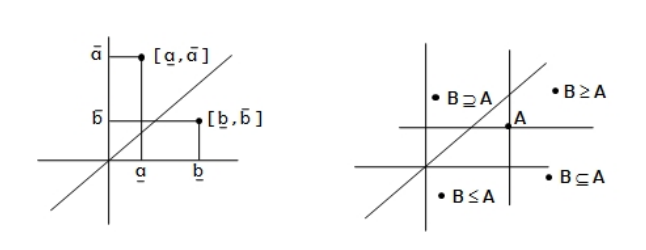
\includegraphics[scale=0.5]{images/florez11.png}
\caption{La primera imagen nos muestra la representación de los intervalos modales y la segunda las inclusiones y las desigualdades.}
\end{figure}

\newpage
Las operaciones{ \em meet} y{ \em join} en $I^*(\mathbb{R})$ para una familia acotada de intervalos modales $A(I) := \{ A(i) = [a_1(i),a_2(i)] \in I^*(\mathbb{R}) : i \in I \}$, donde $I$ es el el dominio de índices, se definen por
\begin{equation}
\wedge(i,I) A(i) = A \in I^*(\mathbb{R}) \text{ es  tal que } \forall (i,I) X \subset A(i) \iff X \subset A,
\nonumber
\end{equation}
\begin{equation}
\vee(i,I) A(i) = B \in I^*(\mathbb{R}) \text{ es  tal que } \forall (i,I) X \supset A(i) \iff X \supset B.
\nonumber
\end{equation}
notado como $(A \wedge B)$ y $(A \vee B)$ para el caso correspondiente. El resultado, visto como función de los límites de los intervalos, es
\begin{equation}
\bigwedge_{i \in I} A(i) = [\max_{i \in I} a_1(i), \min_{i \in I} a_2(i)],
\nonumber
\end{equation}
\begin{equation}
\bigvee_{i \in I} A(i) = [\min_{i \in I} a_1(i), \max_{i \in I} a_2(i)].
\nonumber
\end{equation}

Con estas operaciones el conjunto de intervalos modales es un retículo para la $\subset$-relación, mientras que los intervalos clásicos no lo son, por tanto, estamos completando el conjunto de los intervalos clásicos.

Ambos operadores son isotónicos, i.e.,  si $A_i \subset B_i$ para cada $i \in I$, entonces
\begin{equation}
\bigwedge_{i \in I} A_i \subset \bigwedge_{i \in I} B_i,
\nonumber
\end{equation}
\begin{equation}
\bigvee_{i \in I} A_i \subset \bigvee_{i \in I} B_i.
\nonumber
\end{equation}

En el conjunto de los números conocemos que hay dos relaciones $\leq$ y $\geq$, y las extensiones de estas relaciones a los intervalos se definen por
\begin{equation}
[x_1,x_2] \leq [y_1,y_2] \iff x_i \leq y_i \hspace{0.5cm} i = 1,2.
\nonumber
\end{equation}
Lo que nos conduce a los operadores $\min$ y $\max$ para una familia acotada de intervalos modales $A(I) := \{ A(i) \in I^*(\mathbb{R}) : i \in I \}$ como:
\begin{equation}
\min_{i \in I} A(i) = A \in I^*(\mathbb{R}) \text{ es  tal que } \forall (i,I) X \leq A(i) \iff X \leq A
\nonumber
\end{equation}
\begin{equation}
\max_{i \in I} A(i) = B \in I^*(\mathbb{R}) \text{ es  tal que } \forall (i,I) X \geq A(i) \iff X \geq B
\nonumber
\end{equation}
Computacionalmente expresado:
\begin{equation}
\min_{i \in I} A(i) = [\min_{i \in I} a_1(i), \min_{i \in I} a_2(i)]
\nonumber
\end{equation}
\begin{equation}
\max_{i \in I} A(i) = [\max_{i \in I} a_1(i), \max_{i \in I} a_2(i)]
\nonumber
\end{equation}

El conjunto de los intervalos modales es, por tanto, un retículo bajo la $\leq$-relación. La siguiente figura nos muestra la representación geométrica de los operadores que hemos definido para dos intervalos.
\begin{figure}[h]
\centering
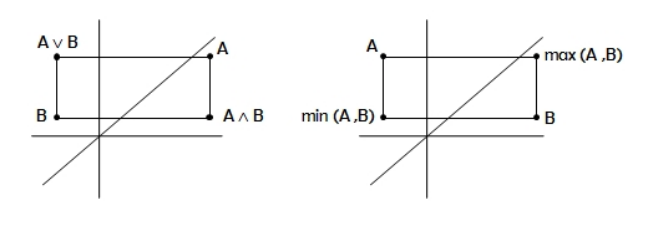
\includegraphics[scale=0.5]{images/florez12.png}
\end{figure}

\subsection{Extensiones semánticas}

En la teoría clásica de Análisis de Intervalos una extensión de una función de $\mathbb{R}^n$ a $\mathbb{R}$ dada por $z = f(x_1, \dotso, x_n)$ es el intervalo de extensión unida $R_f$ de $f$. Para el intervalo $X' = (X_1',\dotso, X_n') \in I(\mathbb{R}^n)$ se define el rango de $f$-valores en $X'$ como
\begin{equation}
R_f(X_1',\dotso, X_n') := \{ f(x_1, \dotso, x_n) : x_i \in X_i' \ \forall i \in \{1, \dotso, n \} \} =
\nonumber
\end{equation}
\begin{equation}
[\min \{ f(x_1, \dotso, x_n) : x_i \in X_i' \ \forall i \in \{1, \dotso, n \} \}, \max \{ f(x_1, \dotso, x_n) : x_i \in X_i' \ \forall i \in \{1, \dotso, n \} \}].
\nonumber
\end{equation}

Para obtener la estimación para la extensión unida, las extensiones racionales del intervalo teórico $fR(X_1', \dotso, X_n')$ se definen como su correspondiente función real-racional $f(x_1, \dotso, x_n)$ reemplazando:
\begin{enumerate}
\item Los argumentos numéricos $x_i$ por sus argumentos de intervalos $X_i'$.
\item Los operadores aritméticos{ \em reales} $\omega$ por su correspondiente operación entre intervalos la cual, en los casos más comunes de computaciones truncadas de cualquier aritmética tiene que dirigirse al exterior $\omega^R$ debido a la inclusión
$$X' \omega Y' \subset X' \omega^R Y' := Out(X' \omega Y'),$$
donde $Out$ representa el redondeo exterior del intervalo $X' \omega Y'$.
\end{enumerate}

Las funciones de intervalos racionales tienen la propiedad, fundamental para todo el cuerpo de Análisis de Intervalos, de ser inclusiva, esto es, para un conjunto de intervalos cumpliendo $X_1' \subset Y_1', \dotso, X_n' \subset Y_n'$ se cumple
\begin{equation}
f R(X_1', \dotso, X_n') \subset f R(Y_1', \dotso, Y_n').
\nonumber
\end{equation}
Suponiendo que no ocurre  ninguna división entre un intervalo que contenga al cero.

La relación entre ambas extensiones es
\begin{equation}
R_f(X_1', \dotso, X_n') \subset f R(X_1', \dotso, X_n').
\nonumber
\end{equation}
Donde $f R$ es computable a parir de los límites de los intervalos $X_1', \dotso, X_n'$ y normalmente representan una sobrestimación de $R_f(X_1', \dotso, X_n')$.

En el Análisis de Intervalos Modales, un rol similar al de $R_f$ se ve cubierto de forma semántica por las funciones * y **, denotadas por $f^*$ y $f^{**}$ (funciones estrella y doble estrella) y definidas por:
\begin{equation}
f^*(X) := \bigvee_{x_p \in X_p'} \bigwedge_{x_i \in X_i'} [f(x_p,x_i),f(x_p,x_i)] = \left[ \min_{x_p \in X_p'} \max_{x_i \in X_i'} f(x_p,x_i), \max_{x_p \in X_p'} \min_{x_i \in X_i'} f(x_p,x_i) \right]
\nonumber
\end{equation}
\begin{equation}
f^{**}(X) := \bigwedge_{x_i \in X_i'} \bigvee_{x_p \in X_p'} [f(x_p,x_i),f(x_p,x_i)] = \left[ \max_{x_p \in X_p'} \min_{x_i \in X_i'} f(x_p,x_i), \min_{x_p \in X_p'} \max_{x_i \in X_i'} f(x_p,x_i) \right]
\nonumber
\end{equation}
Las cuales tienen, por supuesto, la propiedad de inclusión $f^*(X) \subset f^{**}(X)$. Además
\begin{equation}
X \subset Y \Rightarrow f^*(X) \subset f^*(Y) \ \text{ y } \ f^{**}(X) \subset f^{**}(Y).
\nonumber
\end{equation}
En algunos casos puede ocurrir que $f^* \equiv f^{**}$.

Los próximos teoremas nos dan una interpretación lógica de las extensiones semánticas.

\begin{theorem}{\textbf{Teorema de la semántica *:}}\label{theorem1}
Sea $X \in I^*(\mathbb{R}^n)$ y $Z \in I^*(,\mathbb{R})$, se tiene
$$f^*(X) \subset Z \iff \forall(x_p, X_p') \ Q(z,Z) \ \exists (x_i,X_i') \ z = f(x_p,x_i).$$
\end{theorem}

\begin{theorem}{\textbf{Teorema de la semántica **:}}\label{theorem2}
Sea $X \in I^*(\mathbb{R}^n)$ y $Z \in I^*(,\mathbb{R})$, se tiene
$$f^*(X) \supset Z \iff \forall(x_i, X_i') \ Q(z,Dual(Z)) \ \exists (x_p,X_p') \ z = f(x_p,x_i).$$
\end{theorem}

Esto significa que es posible reducir una expresión lógica a inclusiones entre intervalos. Ambos teoremas hacen equivalente una fórmula lógica, con intervalos y predicados funcionales donde los cuantificadores universales preceden a los existenciales, a una inclusión de intervalos.

Por ejemplo, la función real $f(x,y) = x+y$ con los intervalos $X = [1,3]$ e $Y = [2,3]$ el resultado es $X + Y = [4,5]$. De acuerdo al teorema de la semántica * obtenemos
$$\forall(x,[1,3]')\exists(z,[4,5]')\exists(y,[2,3]')x+y=z.$$
Y de acuerdo al teorema de la semántica ** obtenemos
$$\forall(y,[2,3]')\exists(z,[4,5]')\exists(x,[1,3]')x+y=z.$$

Incluso pensando que las funciones $f^*$ y $f^{**}$ son óptimas en el sentido semántico, estos teoremas no explicitan el proceso de computación del intervalo $Z$ que verifica $f^* \subset Z$ ó $f^{**} \supset Z$, i.e., intervalos que son una estimación exterior e interior de $f^*$ y $f^{**}$ respectivamente. De hecho, exceptuando los operadores aritméticos, el cálculo de $f^*$ y $f^{**}$  no se puede lograr mediante computación directa. Si la función continua $f$ es una función racional, entonces existe  una extensión modal racional que se obtiene usando el programa computacional definido por el árbol sintáctico de las expresiones de la función:

\begin{itemize}
\item Si $f$ es una función racional de $\mathbb{R}^n$ a $\mathbb{R}$, entonces su extensión modal racional a los intervalos modales $X_1, \dotso, X_n$ representada por $f \ R(X_1, \dotso, X_n)$ es la función $f \ R$ de $I^*(\mathbb{R}^n)$ a $I^*(\mathbb{R})$ definida por el programa computacional indicado por la sintaxis de $f$ cuando el operador ral se transforma en su extensión semántica.
\end{itemize}

Las funciones de intervalos modales racionales no son interpretables, pero tiene la propiedad de ser isotónicas, i. e., para intervalos $X_1 \subset Y_1, \dotso, X_n \subset Y_n$ se verifica la relación
\begin{equation}
f \ R(X_1, \dotso, X_n) \subset f \ R(Y_1, \dotso, Y_n).
\nonumber
\end{equation}
Asumiendo que no se producen divisiones por intervalos que contengan al cero.

\subsection{Interpretabilidad y optimalidad}

La solución al problema de computar las extensiones semánticas $f^*$ y $f^{**}$ consiste en relacionarlo mediante relaciones de inclusión a algunas extensiones racionales. Las computaciones con $f \ R(X)$ deben de hacerse con truncación externa de cada operador para obtener $f^*(X) \subset f \ R(X)$ y con la truncación interna obtenemos $f \ R(X) \subset f^{**}(X)$. En muchos de los casos la extensión racional $f \ R(X)$ es óptima, i. e.,
\begin{equation}
f^*(X) = f \ R(X) = f^{**}(X).
\nonumber
\end{equation}
Y, exceptuando el redondeo, ambos teoremas semánticos son aplicables al intervalo $f \ R(X)$ proporcionándole un significado lógico a éste.

El Análisis de Intervalos Modales nos proporciona una serie de resultados sobre inclusiones o igualdades que resuelven parte del problema doble de interpretabilidad de extensiones modales racionales y computabilidad de las expresiones semánticas. Ahora mostraremos varios teoremas que nos muestran resultados sobre la interpretabilidad de extensiones racionales.

\begin{theorem}{\textbf{* interpretabilidad de funciones modales racionales:}}\label{th1}
Si las componentes impropias de $X$ son uni-incidentes en $f \ R(X)$ y si $Out(f \ R(Prop(X)))$ existe, entonces
$$Out(f \ R(X)) \supset f^*(X).$$
Donde $Out$ representa el redondeo exterior del intervalo $f \ R(X)$.
\end{theorem}

\begin{theorem}{\textbf{** interpretabilidad de las funciones modales racionales:}}\label{th2}
Si las componentes propias de $X$ son uni-incidentes en $f R(X)$ y si $Out(f \ R(Prop(X)))$, entonces
$$Inn(f \ R(X)) \subset f^{**}(X).$$
Donde $Inn$ representa el redondeo interno del intervalo $f \ R(X)$.
\end{theorem}

Una función real $f$ se llama $x$-totalmente monótona para una variable multi-incidente $x \in \mathbb{R}$ si es uniformemente monótona para esta variable y para cada una de sus incidencias, consideradas como variables independientes.

\begin{theorem}{\textbf{* interpretabilidad con monotonía total:}}\label{th3}
Sea $X$ un vector intervalo y $f \ R$ definido en $Prop(X)$ y totalmente monótona para un subconjunto $Z$ de componentes multi-incidentes. Sea $X \ Dt^*$ el vector agrandado de $X$, esto es, cada incidencia de cada componente multi-incidente del subconjunto con monotonía total está incluida en $X \ Dt^*$ como una componente independiente, pero transformada en su dual si el correspondiente punto incidente tiene un sentido monótono contrario al global de la correspondiente componente $Z$. Para el resto, las componentes impropias muti-indicentes se transforman en un intervalo puntual definido por cualquiera de sus puntos. Entonces
$$f^*(X) \subset f \ R(X \ Dt^*).$$
\end{theorem}

\begin{theorem}{\textbf{** interpretabilidad con monotonía total:}}\label{th4}
Sea $X$ un vector intervalo y $f \ R$ definido en $Prop(X)$ y totalmente monótona para un subconjunto $Z$ de componentes multi-incidentes. Sea $X \ Dt^{**}$ el vector agrandado de $X$, esto es, cada incidencia de cada componente multi-incidente del subconjunto con monotonía total está incluida en $X \ Dt^{**}$ como una componente independiente, pero transformada en su dual si el correspondiente punto incidente tiene un sentido monótono contrario al global de la correspondiente componente $Z$. Para el resto, las componentes propias muti-indicentes se transforman en un intervalo puntual definido por cualquiera de sus puntos. Entonces
$$f^{**}(X) \supset f \ R(X \ Dt^{**}).$$
\end{theorem}

\begin{theorem}{\textbf{Interpretabilidad en el caso general multi-incidente:}}\label{th5}
Si $f \ R(X)$ tiene componentes multi-incidentes impropias y $Xt^*$ se obtiene reemplazando tales componentes por intervalos puntual definido por cualesquiera de sus puntos  de sus dominios, entonces
$$f^*(X) \subset f \ R(X \ t^*).$$
\end{theorem}

Este teorema es útil cuando no es posible realizar test de monotonía.

Es posible obtener mejores resultados si se aplica el concepto de optimalidad.

\begin{definition}
Una función modal racional $f \ R(X)$ se dice óptima si cualquiera de sus operadores no uniformemente monótonos es seguido por operadores de una única variable.
\end{definition}

\begin{theorem}{\textbf{Coerción a la optimalidad:}}\label{th6}
Sean $X$, $f \ R$ y $X \ D$ definidos bajo las condiciones de los teoremas \ref{th3} y \ref{th4}. Y sea $f \ R$ óptimo en $Prop(X)$. En tal caso
$$f^*(X) = f \ R(X \ D) = f^{**}(X).$$
\end{theorem}

Este teorema es útil para resolver el problema, especialmente en el caso cuando la función de la fórmula lógica verifica las condiciones de optimalidad ya que, en este caso, la computación de $f \ R(X \ D)$ es igual a $f^*(X)$, excepto por el redondeo, y el teorema \ref{theorem1} lo hace equivalente a la fórmula lógica.

\textbf{Ejemplo:}

Consideremos una función continua $f : \mathbb{R^2} \to \mathbb{R}$ definida por
$$f(x,y) = \frac{xy}{x+y},$$
con $X = [2,3]$ e $Y = [4,3]$.

La función $f$ es totalmente monótona respecto de $x$ y de $y$ ya que sus derivadas parciales son mayores que cero en los dominios de las variables. Tomando las componentes multi-incidentes como componentes independientes, es decir,
$$f(x_1,x_2,y_1,y_2) = \frac{x_1 y_1}{x_2 + y_2},$$
se tiene que:
$$\frac{\partial f}{\partial x_1} > 0, \hspace{0.5cm} \frac{\partial f}{\partial x_2} < 0, \hspace{0.5cm} \frac{\partial f}{\partial y_1} > 0 \hspace{0.5cm} \text{y} \hspace{0.5cm} \frac{\partial f}{\partial y_2} > 0.$$

Con estas condiciones mostraremos las aplicaciones de tres teoremas:
\begin{enumerate}
\item De acuerdo al teorema \ref{th5} las componentes impropias multi-incidentes se reemplazan por intervalos puntual, $Xt^* = ([2,3],[4,4],[2,3],[4,4])$ el resultado es
$$f \ R(Xt^*) = \frac{X \ [4,4]}{X + [4,4]} = [1.1428,2].$$
\item De acuerdo al teorema \ref{th3} tenemos $X \ Dt^* = ([2,3],[4,4],[3,2],[4,4])$ y el resultado es
$$f \ R(X \ Dt^*) = \frac{X \ [4,4]}{Dual(X) + [4,4]} = [1.3333,1.7144].$$
\item De acuerdo al teorema \ref{th6} tenemos $X \ D = ([2,3],[4,3],[3,2],[3,4])$ y el resultado es
$$f^*(X) = \frac{X Y}{Dual(X) + Dual(Y)} = [1.3333,1.5].$$
\end{enumerate}

La mejor aproximación se obtiene mediante el teorema \ref{th6}. En el lado contrario tenemos la aproximación obtenida mediante el teorema \ref{th5}. En este ejemplo es
$$f^*(X) \subset f \ R(X \ Dt^*) \subset f \ R(Xt^*).$$

\section{Conclusiones}

En este capítulo hemos definido e introducido las diferentes propiedades del Análisis de Intervalos. Como hemos explicado, la Aritmética de Intervalos se puede aplicar a diversos campos de investigación para solucionar los problemas de redondeo. Por supuesto las gráficas por ordenador no iban a ser una excepción.

También hay una visión del Análisis de Intervalos Modales, que completa la definición clásica de Análisis de Intervalos mediante aplicación de los cuantificadores a la definición de intervalo. La teoría de Intervalos Modales nos da los intervalos impropios que en la teoría clásica carece de sentido y, en la mayoría de casos, la transformación lleva tal intervalo impropio en uno propio sin explicación lógica. El Análisis de Intervalos Modales nos concede una explicación para tales casos por medio de las aplicaciones de los teoremas incluidos en este capítulo.

Los teoremas desarrollados son la base para la teoría de Intervalos Modales y, además, nos ayudarán a mejorar el Ray Tracing, o trazado, de superficies implícitas.
\chapter{Aplicaciones del Análisis de Intervalos a las superficies implícitas}

Como ya hemos explicado en el capítulo anterior, el Análisis de Intervalos es una herramienta bastante fiable con respecto a los problemas de redondeo de los ordenadores. Además tiene aplicaciones en muchas áreas como:
\begin{itemize}
	\item Gráficas por ordenador.
	\item Detección de colisiones.
	\item Errores de aproximación en la transferencia de datos entre sistemas CAD/CAM.
	\item Ray Tracing de superficies paramétricas.
	\item Ray Tracing de superficies implícitas.
\end{itemize}

El Análisis de Intervalos ha sido usado en Infografía en especial para la creación de algoritmos de subdivisión fidedignos. Estos algoritmos pueden evaluar áreas o espacio para detectar la{ \em existencia} de superficies o curvas. Esto permite la creación de estructuras como árboles octales o cuaternarios, octrees y quadtrees en inglés de forma respectiva.

Este capítulo comienza con la introducción de diferentes algoritmos de subdivisión de intervalos. A continuación presentamos diferentes técnicas para desarrollar Ray Tracing, centrándonos en las basadas en Aritmética de Intervalos. Finalmente se incluye una comparación entre aproximaciones basadas en intervalos para encontrar las raíces de las intersecciones para conocer la eficiencia.

\section{Algoritmos de subdivisión recursiva}

Existen infinidad de técnicas para representar objetos geométricos como representaciones poligonales, técnicas de subdivisión espaciales, parches paramétricos... El proceso de visualización mediante Análisis de Intervalos conbina características de de todos las técnicas nombradas, aunque la más común suele ser la subdivisión del espacio. Éste es usado para representar objetos geométricamente  y luego aplicar estrategias de renderizado como el Ray Tracing.

Los métodos de subdivisión del espacio tienen como propósito{ \em encerrar} al objeto.  Esto es, por ejemplo en el método de los árboles octales, si una región cúbica encierra un objeto entonces podemos dividir el cubo en ocho octantes iguales. Cada nuevo cubo, u octante, es evaluado para asegurarnos que contiene alguna parte del objeto. Este proceso continua hasta un nivel predefinido de subdivisión.
\\Este proceso crea una estructura octal con información sobre el objeto que puede ser utilizada para crear una visualización directa o acelerar otras técnicas de visualización.

\subsection{Subdivisión espacial usando Aritmética de Intervalos}

El algoritmo de a subdivisión se basa en la subdivisión recursiva del espacio que contiene al objeto para generar ocho cubos llamados octantes.

Un octante consiste en una región cúbica definida por tres intervalos, en el que cada uno de ellos representa los valores de frontera del octante en cada una de las dimensiones. Los octantes que no contienen ningún punto de la superficie son descartados.

Este proceso permite la creación de estructuras que describan el objeto de forma geométrica. La creación de estructuras como los árboles octales es directa. Un árbol octal es un tipo de estructura  que representa el espacio ocupado por varios objetos en una escena tridimensional. La versión bidimensional es llamado árbol cuaternario.

En conclusión estamos ante un tipo de árbol en el que cada nodo representa regiones y sus hojas son regiones aún más pequeñas que contienen parte de los objetos

Es posible usar este algoritmo para representar operaciones entre diferentes funciones implícitas. Por ejemplo, Suffern et al.\cite{Suffern03} introdujo una técnica para renderizar la intersección entre dos superficies implícitas basada en un árbol octal. Esta técnica usaba Aritmética de Intervalos para descartar regiones que no contenían alguna de ambas superficies. Si la región contiene a ambas superficies se subdivide y se repite el mismo análisis.

Los octantes que contienen alguna parte de la superficie se subdividen en otras ocho regiones que se evalúan para saber si siguen conteniendo alguna parte de la superficie.

Dada una superficie implícita, definida por $f(x,y,z) = 0$, y una región cúbica definida por tres intervalos $X$, $Y$ y $Z$. Usaremos la extensión unida de $f$ definida en el capítulo anterior para saber si la superficie interseca a la región cúbica. A esta extensión la denotaremos por $F(X,Y,Z)$.

El algoritmo funciona como sigue: Si $0 \in F(X,Y,Z)$ significa que la región interseca a al superficie, en caso contrario, la región puede descartarse.

Las regiones del espacio que contienen parte de la superficie se subdividen de forma recursiva y se evalúan de nuevo hasta que alcanzamos el tamaño de mallado deseado, el cual habremos seleccionado en base a la resolución que necesitemos. Al final del algoritmo tendremos una lista de cubos que contienen partes de la superficie, pero parte de esos cubos contendrán regiones que no son solución a nuestro problema. El algoritmo de subdivisión usando funciones inclusión sería el siguiente:
\begin{verbatim}
Evaluate(X,Y,Z):
   If(0 belongs to F(X,Y,Z))
      If(X or Y or Z <= Threshold)
         Add (X,Y,Z) to solution list
      Else
         Subdivide X into X_1 and X_2
         Subdivide Y into Y_1 and Y_2
         Subdivide Z into Z_1 and Z_2
         Evaluate (X_i,Y_j,Z_k) for i,j,k in {1,2}
   Else
      The octant is rejected
\end{verbatim}

Este algoritmo tiene muchas debilidades. La principal es que el algoritmo es muy dependiente del número de subdivisiones requeridas para alcanzar la resolución deseada, lo que provoca un gran coste computacional.

Aunque este algoritmo es muy útil en el caso tridimensional se puede usar para casos bidimensionales e incluso para rasterizar curvas algebraicas, véase \cite{Oliveira00,Taubin94}.

\subsection{Mejorando el proceso de subdivisión}

Existen muchas técnicas para mejorar el proceso de subdivisión. El principal objetivo de tales técnicas es permitir el diseño de algoritmos de subdivisión más eficientes y robustos.

Una versión adaptativa del algoritmo trabaja con la curvatura de la superficie durante el propio proceso de subdivisión. Balsys et al. \cite{Balsys01} desarrollaron un algoritmo adaptativo para mejorar la creación de la estructura del árbol octal. Esto soluciona los problemas surgidos por la diferencias de profundidad entre nodos adyacentes.

En \cite{Oliveira00,Suffern03} las técnicas adaptativas se usan para garantizar que las subdivisiones son lo suficientemente pequeñas como para contener partes de una curva con una curvatura relativamente grande. Esto se consigue evaluando el gradiente de la curva en cada subdivisión: un gradiente muy grande significa que la curva varía mucho dentro de la región en la que estamos trabajando. Por tanto tenemos que generar cubos pequeños para representar la curvatura.

Carvalho et al.\cite{Carvalho98} proporcionó ciertas condiciones para detener el proceso de subdivisión recursiva cuando las celdas son lo suficientemente pequeñas y no contienen intersecciones cerradas de la curva.

Bühler\cite{Buhler02} desarrolló una estimación lineal implícita basada en intervalos, ILIE por su siglas en inglés, que consiste en un cierre lineal de un objeto adaptado a la topología intrínseca del mismo. Cada celda se reduce a partes que sólo contienen la correspondiente ILIE, lo que reduce el número de subdivisiones del proceso total. Esto, por supuesto, reduce el tiempo de computación.

Standder y Hart\cite{Stander97} nos muestran cómo los puntos críticos de la función afectan a la topología de la superficie implícita. Usaron la Aritmética de Intervalos para encontrar tales puntos y, tras esto, modificaron la poligonalización para acomodarla a los cambios topológicos.

Duff\cite{Duff92} desarrolló una aplicación geométrica de los intervalos usando árboles en donde las hojas son funciones implícitas. El algoritmo tiene en cuenta la información del árbol completo en cada subdivisión, obteniendo así una escena completa con varios objetos correctamente renderizados en la misma escena.

\section{Ray Tracing eficiente aplicado a superficies implícitas}

En esta sección abarcaremos distintas mejoras desarrolladas por distintos autores para realizar un Ray Tracing eficiente en superficies implícitas. Estos trabajos se centran en la creación de intersecciones fidedignas. Los autores aplican distintas técnicas numéricas para controlar la pérdida de raíces debido al uso de algoritmos basados en números de coma flotante. Esto puede generar que ciertas partes de las superficies más{ \em finas} puedan perderse durante el proceso de renderización. Aunque este tipo de superficies son casos especiales  sería deseable obtener un método que también fuera capaz de cubrir estos casos.

Otro problema relacionado con el Ray Tracing  es la eficiencia de los algoritmos. Whitted\cite{Whitted80} menciona que el 95 por ciento del gasto de tiempo de renderizado era debido a las intersecciones en escenas complejas. El Ray Tracing es lento debido a que necesita de muchas intersecciones para cada píxel. Esto se incrementa en las superficies implícitas e incluso más con la Aritmética de Intervalos.

\subsection{Aproximación por muestreo puntual}

Los test de intersección se pueden desarrollar en dos pasos:
\begin{enumerate}
\item Encontrar la raíz, en donde el primer intervalo que la contiene es seleccionado.
\item Refinamiento de la raíz, en donde el intervalo que la contiene se reduce hasta llegar a un tamaño prefijado.
\end{enumerate}

La clave en el primer paso es garantizar que el intervalo contiene una única raíz de la función implícita. Este paso normalmente es más complicado y puede resolverse con métodos como el de la bisección. Sin embargo, este método puede causar problemas como la convergencia a la raíz equivocada o, directamente, la no convergencia.
\begin{verbatim}
Bisection(t_1,t_2):
   t_m = (t_1 + t_2)/2   
   If(f(t_m) == 0)
      t_m is a root
   Else
      If(abs(t_2 - t_1) < Threshold)
         There are no roots
      Elif(f(t_1)*f(t_m) < 0)
         Bisection(t_1,t_m)
      Else
         Bisection(t_m,t_2)
\end{verbatim}

Una alternativa al método de la bisección es el método de Newton, el cual tiene la ventaja de que, en caso de converger, lo hace de forma cuadrática en lugar de lineal como el método de la bisección. Sin embargo, el método de Newton puede no converger a ninguna de las raíces o, en algunos casos, divergir\cite{Hart01}.

Un ejemplo de los problemas del muestreo puntual es el de la imagen \ref{florez45}. Si los intervalos iniciales son demasiado grandes, imagen a), se pierde mucha información y, por tanto, raíces. Si usamos un tamaño más pequeño de intervalos el problema no se resuelve del todo, como se puede ver en b). Además, intervalos pequeños significan pérdida de eficiencia. El problema se soluciona usando Aritmética de Intervalos, casos c) y d). Incluso usando una precisión pequeña en el método de la bisección, caso c), el resultado es mejor que en los anteriores. El mejor resultado posible sería el d) que es cuando el método de la bisección alcanza la precisión de máquina.
\begin{figure}[h]
	\centering
	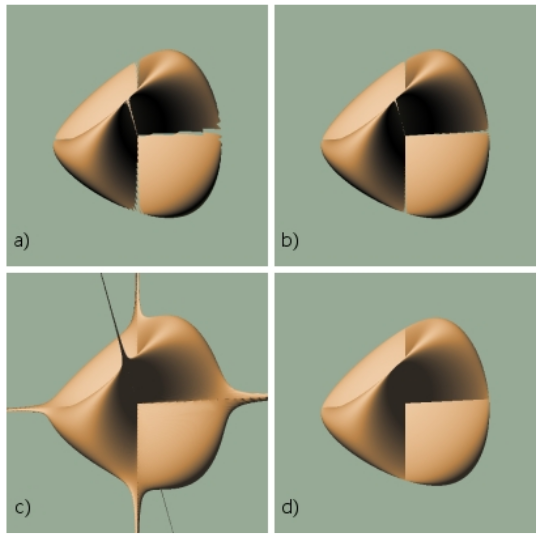
\includegraphics[scale=0.5]{images/florez5.png}
	\caption{Imágenes obtenidas por muestreo puntual. a) Sin Aritmética de Intervalos e intervalo de tamaño 0.001. b) Sin Aritmética de Intervalos e intervalo de tamaño 0.0001. c) Con Aritmética de Intervalos y bisección con precisión 0.0001. d) Con Aritmética de Intervalos y bisección con precisión máquina.}
	\label{florez45}
\end{figure}

\subsection{Aproximación por Aritmética de Intervalos}

Mitchell\cite{Mitchell90} propuso el uso de Aritmética de Intervalos para encontrar la raíz de una forma segura. La extensión unida de la función intersección $f$ es
\begin{equation}
F(T) = f(c_x + T(x_s - c_x), c_y + T(y_s - c_y), c_z + T(y_z - c_z)).
\nonumber
\end{equation}
Los valores $c_x$, $c_y$ y $c_z$ indica el punto de vista del observador y los valores $x_s$, $y_s$ y $z_s$ indican el punto donde el rayo interseca la pantalla y $T$ es el parámetro del intervalo. La diferencia con la definición clásica es el uso del parámetro del intervalo $T$, que toma intervalos como valores en lugar de puntos reales.

La ecuación anterior se conoce por{ \em función inclusión} para la superficie implícita. Esta función puede ser evaluada usando cualquier intervalo de $T$. Si el resultado de la evaluación es $0 \notin F(T)$ podemos asegurar que no hay ninguna raíz de $f$ en el valor actual de $T$. Aún así esta función no consigue el resultado contrario, esto es, para conocer si existen raíces para cada valor de $T$. Esto es debido a que en cada operación los límites del intervalo se redondean al alza y a la baja para garantizar que cualquier resultado posible no se pierda. Este redondeo incluye valores que no son parte de la evaluación de la función, por ello el cero puede ser incluido mediante cualquiera de las operaciones de redondeo. Por tanto, la función inclusión se usa como función descarte. 

Para saber si hay una única raíz en el intervalo usamos la extensión unida $F'$ de la derivada $f'$. El algoritmo propuesto por Mitchell es el siguiente:
\begin{verbatim}
Mitchell(T as [t_1,t_2]):
   If(0 not in F(T))
      If()
         If(f(t_1)*f(t_2) <= 0)
            Root refinement over T using Bisection or Newthon method
      Else
         T_1 = [t_1,(t_1 + t_2)/2]
         T_2 = [(t_1 + t_2)/2,t_1]
         
         If(width(T_1) >= threshold)
            Mitchell(T_1)
         Else
            Root refinement over T_1 using Bisection or Newthon method
         
         If(width(T_2) >= threshold)
            Mitchell(T_2)
         Else
            Root refinement over T_2 using Bisection or Newthon method
   Else
      Reject T
\end{verbatim}

El algoritmo comienza evaluando el intervalo $T$ usando la función inclusión. En el caso de que el cero esté contenido en el resultado, la derivada de la función implícita es se evalúa usando el valor del intervalo de $T$. Si el cero no pertenece al resultado de la evaluación de la derivada se comprueba que los valores de los extremos del intervalo sean de signo contrario y, en caso de darse, sabemos que sólo hay una sola raíz en el intervalo $T$. Por tanto podríamos realizar el proceso de refinamiento del intervalo.
\\En el caso de que al evaluar la función inclusión y la derivada el cero esté contenido, subdividimos el intervalo $T$ en dos y repetimos el proceso con los nuevos intervalos.

Otra consideración a tener en cuenta es la anchura que a la que los intervalos pueden llegar a alcanzar antes de finalizar la búsqueda de la raíz y comenzar el refinamiento del intervalo. Por ejemplo, cuando las raíces se encuentran en la tangente, la convergencia será siempre hacia estas raíces. En tal caso, la derivada es siempre cero y el proceso siempre termina cuando se alcanza un valor mínimo de anchura.

En otros casos no hay garantía de que el mínimo de anchura permitido contenga alguna raíz. En tal caso se puede establecer el mínimo en la precisión del ordenador, lo que incrementa significativamente las probabilidades de que contenga una raíz\cite{Capriani00}.

Mitchell no usó redondeo en sus operaciones entre intervalos. Consideraba que el uso de coma flotante en la aritmética proporcionaba suficiente precisión para la renderización de las superficies. La razón que esgrimía era que la Aritmética de Intervalos era que aumentaba el tiempo de renderización.

Finalmente, este algoritmo propone resolver el refinamiento del intervalo usando técnicas clásicas como ĺos métodos de bisección, Newton o cualquier otro suficientemente rápido para renderizar las superficies. Esto es debido a que, según Mitchell, La Aritmética de Intervalos es demasiado lenta para realizar este proceso.

\subsection{Mejorando la aproximación por Aritmética de Intervalos}

Si el algoritmo para encontrar la raíz se desarrolla usando la bisección clásica de intervalos, mismo algoritmo que en la sección anterior pero sin la verificación de la derivada, la eficiencia del algoritmo puede bajar drásticamente.

Capriani et al. \cite{Capriani00} nos muestran que hay algoritmos basados en intervalos para encontrar raíces eficaces y suficientemente rápidos como para renderizar una superficie implícita.
\begin{verbatim}
Newton(T as [t_1,t_2]):
   If(0 in F(T))
      If(0 not in F'(T))
         t_m = t_1 + midpoint(T)
         NT = t_m - f(t_m)/F'(T)
         NTT = NT intersecting with T
        
         If(NTT is empty)
            There's no root
         Else
            Newton(NTT)
        
      Else
         T_1 = [t_1,midpoint(T)]
         T_2 = [midpoint(T), t_2]
         
         If(width(T_1) >= Threshold)
            Newton(T_1)
         Else
            T_1 is the root
            
         If(width(T_2) >= Threshold)
            Newton(T_2)
         Else
            T_2 is the root
   Else
      Reject T
\end{verbatim}

El método de intervalos de Newton es una aproximación muy buena que es más rápida que la versión clásica de la bisección. El método de intervalos de Newton tiene a menudo convergencia cuadrática, pero requiere del cálculo de las derivadas.

Capriani et al. propusieron una importante mejora del método mediante un operador Alefeld-Hansen. El operador es obtenido cuando $0 \in F'(T)$. Si $T = [t_1,t_2]$ se define
\begin{equation}
\frac{1}{F'(T)} = \left\{ \begin{tabular}{l l l}
$\left[ \frac{1}{t_2}, \infty \right]$ & & si $t_1 = 0$, \\ \\
$\left[ - \infty, \frac{1}{t_1} \right]$ & & si $t_2 = 0$, \\ \\
$\left[ - \infty, \frac{1}{t_1} \right] \cup \left[ \frac{1}{t_2}, \infty \right]$ & & Cualquier otro caso.
\end{tabular}
\right.
\nonumber
\end{equation}
Véase \cite{Alefeld70,Hansen78}.

Usando aritmética extendida\cite{Hansen03} el operador es
\begin{equation}
AH(T) = \left[ midpoint(T) - \frac{f(midpoint(T))}{F'(T)} \right] \cap T.
\nonumber
\end{equation}

El operador de Alefeld-Hansen se puede añadir al método de intervalos de Newton para comprobar los casos en los que $0 \in F'(T)$. Como se dice en \cite{Capriani00}, el resultado de la evaluación de este operador puede ser el conjunto vacío, un sólo intervalo o dos intervalos de anchura máxima la mitad del intervalo de partida. Esto significa que el operador tiene convergencia cuadrática en la mayoría de casos. Cuando el operador devuelve dos intervalos ambos deben de ser usados para evaluar la función de forma recursiva. El algoritmo es el siguiente:
\begin{verbatim}
AH(T as [t_1,t_2]):
   If(0 in F(T))
      If(0 not in F'(T))
         t_m = t_1 + midpoint(T)
         NT = t_m - f(t_m)/F'(T)
         NTT = NT intersecting with T
        
         If(NTT is empty)
            There's no root
         Else
            AH(NTT)
       
      Elif(0 not in f(t_m))
         AH(T) = (t_m - f(t_m)/F'(T)) intersecting T
         If(AH(T) = emptyset)
            There's no root
         Else
            If(AH(T) generates one interval T_1)
               AH(T_1)
            Elif(AH(T) generates two intervals T_1 and T_2)
               AH(T_1)
               AH(T_2)
         
      Else
         T_1 = [t_1,midpoint(T)]
         T_2 = [midpoint(T),T_2]         
         
         If(width(T_1) >= Threshold)
            Newton(T_1)
         Else
            T_1 is the root
            
         If(width(T_2) >= Threshold)
            Newton(T_2)
         Else
            T_2 is the root
         
   Else
      Reject T
\end{verbatim}

Los algoritmos previos requerían del uso de derivadas de la función. Esto es una desventaja cuando tenemos que renderizar funciones no derivables. En estos casos podemos usar el método de la bisección clásica es una alternativa que funciona bien a pesar de la falta de eficiencia.

Estrada et al. \cite{Estrada03}  propusieron un algoritmo para optimizar la estrategia base del método de intervalos de la bisección. Básicamente proponen una serie de condiciones que tienen que alcanzarse durante el proceso de bisección. Sostenían que, dado un intervalo $T = [t_1,t_2]$ y su punto medio $t_m$, si $\overline{F([t_1,t_1])*F([t_m,t_m])} \leq 0$ entonces el intervalo $[t_m,t_2]$ se rechaza. Este algoritmo se llama MRF.

En otro algoritmo llamado MRFro \cite{Estrada03} introducen algunas condiciones para mejorar el método de la bisección. Este algoritmo evalúa $F([t_1,t_2])$ solo cuando
$$\underline{F([t_1,t_1])*F([t_2,t_2])} > 0,$$
ya que $\overline{([t_1,t_1])*F([t_2,t_2])} \leq 0$ te asegura que $0 \in F([t_1,t_2])$, lo cual no es verdad si tenemos en cuenta el redondeo. El redondeo puede introducir  valores que verifiquen la ecuación, pero eso no es verdad para los valores originales del intervalo. Sin embargo, esta suposición fue suficiente para las superficies renderizadas en el trabajo de Estrada et al.

\subsection{Comparación de diferentes aproximaciones por intervalos}

Como hemos podido ver en las secciones anteriores hay diferentes maneras de realizar aproximaciones mediante intervalos que nos garanticen cierto nivel de fiabilidad en las intersecciones mediante Ray Tracing. Esta sección cubre una comparación entre la eficiencia  de distintos métodos. Las superficies utilizadas en las pruebas están presentes en la figura \ref{florez49}. Estas superficies fueron renderizadas mediante rayos primarios usando uno por píxel.
\begin{figure}[h]
	\centering
	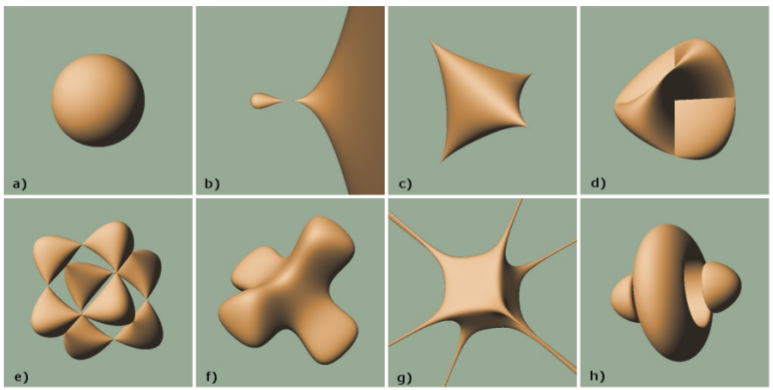
\includegraphics[scale=0.5]{images/florez6.png}
	\caption{Superficies usadas para comparar distintos métodos basados en intervalos para realizar Ray Tracing en superficies implícitas. a) Esfera. b) Superficie{ \em gota}. c) Kusner-Schmitt. d) Crosscap. e) Superficie Chubs. f) Modelo K3 McMullen g) Cubo astado. h) Toro Gumdrop.}
	\label{florez49}
\end{figure}

Como vemos en los resultados que extrae \cite{Florez08}, cinco han sido los métodos analizados: el algoritmo propuesto por Mitchell, el método de Newton basado en intervalos, el método de Newton usando el operador de Alefeld-Hansen, el algoritmo MRFro y un algoritmo que combina las condiciones del MRFro y las del método de Newton basado en intervalos.

\begin{remark}
Los resultados presentados por \cite{Florez08} se basan en imágenes de 300x300 píxeles de resolución  y fueron renderizadas en un ordenador con un procesador Pentium 4.
\end{remark}

\begin{figure}[h]
	\centering
	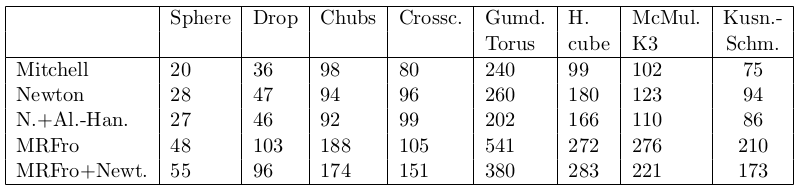
\includegraphics[scale=0.5]{images/florez7.png}
	\caption{Comparación de diferentes métodos.}
	\label{florez41}
\end{figure}

Obviamente los resultados son mejores para la esfera en todos los métodos y peores para una superficie compleja como el toro Gumdrop. El algoritmo de Mitchell muestra una mejor eficiencia para una superficie tan sencilla como es la esfera, pero cuando la complicación va aumentando el mejor método es el de Newton+AH. Además el método de Newton también mejora relativamente la velocidad, pero no lo suficiente. Esto nos indica dos cosas:
\begin{itemize}
\item Las comprobaciones extra que se necesitan en el operador de Alefeld-Jansen se compensa con la mejor convergencia en superficies complejas.
\item En el caso de superficies simples, como la esfera, es mejor aplicar métodos simples como el de Mitchell.
\end{itemize}

El algoritmo MRFro es el más lento en todos y esto es debido a que no toma información extra de la superficie como puede ser la derivada. Cuando se añade información extra, como la subdivisión de Newton, el algoritmo mejora su eficiencia en superficies complejas pero no para superficies simples.

La imagen \ref{florez410} nos muestra gráficamente los resultados de la tabla \ref{florez41}.  Las superficies fueron intencionalmente ordenadas de menos a más computacionalmente costosa.  Esto indica que la complejidad se incrementa de izquierda a derecha. Además un mayor tiempo indica menor eficiencia y viceversa.

Los algoritmos de Mitchell, Newton y Alefeld-Hansen tiene una eficiencia casi lineal cuando la complejidad crece. Además, la eficiencia es parecida en estos tres métodos que usan la derivada como fuente de información.

Por otro lado, el hecho de que tengan una eficiencia tan parecida nos hace darnos cuenta de que podemos usar operaciones con intervalos en todo el proceso sin afectar al tiempo de computación.

\begin{figure}[h]
	\centering
	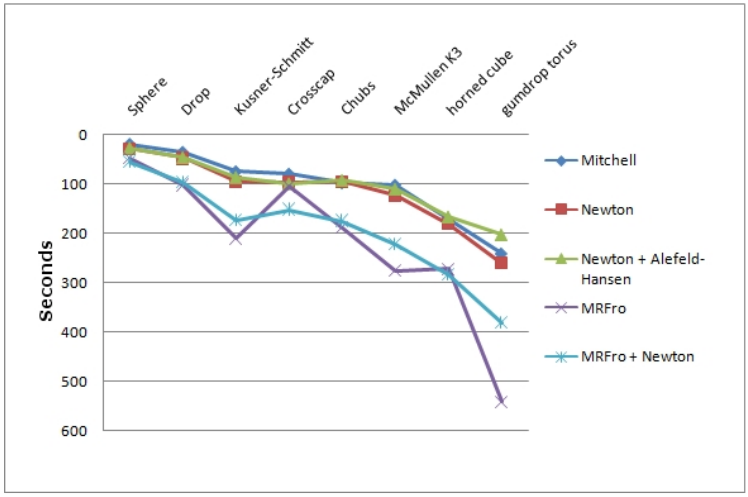
\includegraphics[scale=0.5]{images/florez8.png}
	\caption{Resultados de la comparación de diferentes métodos de Ray Tracing para las superficies analizadas. Las diferencias en calidad de renderización no son apreciables entre los métodos.}
	\label{florez410}
\end{figure}

\subsection{Otras aproximaciones destacables}

\subsubsection{Métodos basados en constantes de Lipschitz}

Dada una función implícita $h(t)$, si existe una constante positiva $L$ tal que para cualesquiera valores $t_1$ y $t_2$ se verifica
\begin{equation}
|h(t_1) - h(t_2)| < L |t_1 - t_2|,
\nonumber
\end{equation}
entonces se dice que $H$ satisface la condición de Lipschitz y $L$ se conoce por el nombre de constante de Lipschitz. Si $t_1$ se encuentra relativamente cerca de $t_2$, entonces
\begin{equation}
\frac{|h(t_1) - h(t_2)|}{|t_1 - t_2|} < L
\nonumber
\end{equation}
representa la derivada de la función $h$. En tal caso $L$ mide la variación de la función entre $t_1$ y $t_2$.

El método de las superficies L-G \cite{Kalra89} se basa en las constantes de Lipschitz para desarrollar un método eficaz y de confianza de Ray Tracing en funciones implícitas. Este método trabaja con dos pasos:
\begin{enumerate}
\item Se crea una estructura octal para la función implícita $f(x)$ con $x \in \mathbb{R}^3$ y y para la que existe una constante de Lipschitz $L$. Sea $x_0$ el centro de uno de los cubos y $d$ la distancia entre éste y cualquiera de los vértices, si $|f(x_0)| > Ld$ entonces podemos descartar el cubo. De otro modo el cubo se subdivide en otros ocho cubos nuevos. La mayoría de cubos se aceptará o rechazará sin problema, pero puede haber casos conflictivos como los que se muestran en la figura \ref{florez411}.
\begin{figure}[h]
	\centering
	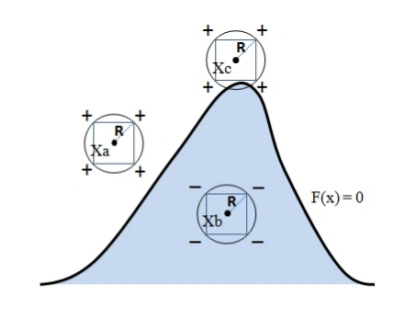
\includegraphics[scale=0.5]{images/florez9.png}
	\caption{Esferas con centro en $x_a$ y $x_b$ no intersecan a la superficie. Mientras que la esfera con centro en $x_c$ puede que sí la interseque.}
	\label{florez411}
\end{figure}

\item Se realiza Ray Tracing sobre la superficie usando la estructura creada en el primer paso. Si ahora consideramos la función intersección $g(t)$ con constante de Lipschitz $G$. Sean $t_1$ y $t_2$ los puntos de entrada de $g$ en un octal, entonces $t_m = \frac{t_1 + t_2}{2}$ y $d = \frac{t_2 - t_1}{2}$. Si $|g(t_m)| > Gd$ entonces existe una única raíz entre $t_1$ y $t_2$. 
\end{enumerate}

El algoritmo sería el que sigue:
\begin{verbatim}
Lipschitz(t_1,t_2):
   Compute G for t_1, t_2
   t_m = midpoint(t_1,t_2)
   d = (t_2 - t_1)/2
   If(abs(t_m) > G*d)
      If(F(t_1)*F(t_2) < 0)
         Compute using Newton
      Else
         There's no intersection
   Else
      Lipschitz(t_1,t_m)
      Lipschitz(t_m,t_2)
\end{verbatim}

Otro método basado en constantes de Lipschitz es el Sphere Tracing\cite{Hart96}. Este método es similar al de las superficies L-G pero usa cotas de Lipschitz en lugar de constantes de Lipschitz. Una cota de Lipschitz es cualquier constante que satisface la condición de Lipschitz, pero no necesariamente la más pequeña. En este método, debemos primero encontrar una cota de Lipschitz para una determinada función según qué distancia consideremos.

\subsubsection{Aritmética afín}

De Cusatis et al.\cite{Cusatis99} introdujeron el uso de aritmética afín al Ray Casting de superficies implícitas. La Aritmética de Intervalos puede generar una sobre estimación en algunas operaciones con intervalos. La Arimética afín se propuso para controlar  esta sobrestimación ya que la aproximación se realiza sobre un paralelogamo, véase \ref{florez413}. La Aritmética afín converge cuadráticamente mientras que la bisección usando Aritmética de Intervalos lo hace de forma lineal.
\begin{figure}[h]
	\centering
	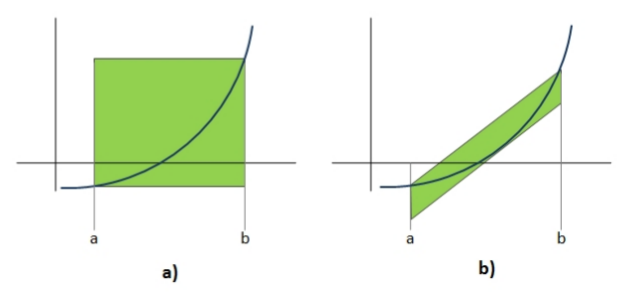
\includegraphics[scale=0.5]{images/florez10.png}
	\caption{Aproximación de una función en un intervalo $[a,b]$. a) Usando Aritmética de Intervalos. b) Usando Aritmética afín.}
	\label{florez413}
\end{figure}

En la Aritmética afín una cantidad $x$ se define mediante la forma afín
\begin{equation}
\hat{x} = x_0 + x_1 \epsilon_1 + \dots + x_n \epsilon_n,
\nonumber
\end{equation}
la cual es un polinomio de grado uno. Los elementos $\epsilon_i$ son desconocidos pero sabemos que oscilan en el intervalo $[-1,1]$. Éstos pueden contribuir a la incertidumbre de dos o más cantidades. Esto indica cierta dependencia subyacente entre las cantidades.

El esquema de este nuevo algoritmo es básicamente el mismo que el que describe este mismo concepto en la Aritmética de Intervalos. La diferencia es qué librería ha de usarse para el cálculo de las extensiones unidas. Como pasa en la Aritmética de Intervalos, las operaciones de aritmética básicas y funciones pueden ser extendidas a formas afines que sean manejables\cite{Stolfi97}.

Sin embargo, las mejoras introducidas por el uso de Aritmética afín van en detrimento del algoritmo básico propuesto por Mitchell\cite{Cusatis99}, pero no en detrimento de en un método más veloz como el de Newton con intervalos. Además, ha sido probado que la Aritmética afín es un caso especial de la forma centrada de la Aritmética de Intervalos\cite{Gavriliu05}.

\section{Conclusiones}

En este capítulo hemos hecho una introducción de diferentes aplicaciones de la Aritmética de Intervalos en la creación de estructuras de subdivisión y también en la creación de test de intersección de Ray Tracing en superficies implícitas. La Aritmética de Intervalos nos proporciona una manera sencilla de comprobar los tres ejes de un cubo para saber si interseca a la superficie. Esta técnica puede ser mejorada mediante el estudio de la superficie para realizar más subdivisiones en secciones críticas de ésta.

Además, también hemos presentado diferentes técnicas para realizar test de intersección entre rayos y superficies implícitas. La mayoría de métodos para los test de intersección están destinados a trabajar con Aritmética de Intervalos, la cual remplaza las operaciones sobre número reales por operaciones sobre intervalos.

Hay diferentes aproximaciones, por ejemplo, las basadas en derivadas y otras que crean ciertas condiciones para mejorar el proceso de bisección. Aunque  el uso de derivadas mejora la eficiencia, puede que ésta no sea fácil de obtener para algunos tipos de superficies implícitas. Dimos también un rápido vistazo a la comparación de distintos métodos para saber su comportamiento y eficiencia ante las mismas superficies con distinta complejidad y vimos que en superficies sencillas son máś eficientes algoritmos sencillos y en superficies complejas es más eficaz el uso de algoritmos algo más complejos debido a que suelen presentar convergencia de orden cuadrático frente a la lineal de los más simples, lo que compensa las comprobaciones extras que deben realizarse.

Finalmente también vimos como hay otra serie de técnicas que no usan Aritmética de Intervalos como las basadas en constantes de Lipschitz o en Aritmética afín. Aunque su perdida de generalidad les hace menos atractivas y, por tanto, su uso está muy poco popularizado.

\nocite{*}
\bibliography{references}\addcontentsline{toc}{chapter}{Bibliografía}
\bibliographystyle{alpha}
%
%\appendix
%\input{apendices/manual_usuario/manual_usuario}
%%\input{apendices/paper/paper}
%\input{glosario/entradas_glosario}
% \addcontentsline{toc}{chapter}{Glosario}
% \printglossary
%\chapter*{}
%\thispagestyle{empty}

\end{document}
